% Copyright (c) 2026 Selina Cheggour. Tous droits réservés. Voir le fichier LICENSE.
\documentclass[11pt,a4paper]{article}
\newcommand{\doctype}{Fiche étudiants}
% Copyright (c) 2026 Selina Cheggour. Tous droits réservés. Voir le fichier LICENSE.
% Style commun des deux documents, repris de BI_ISG/BI/Séance3/GucciMetaverse.tex (palette bleue).
% Chargé par input{../style_bleu} dans guide_selina.tex et fiche_etudiants.tex.
\usepackage[T1]{fontenc}
\usepackage[utf8]{inputenc}
\usepackage[french]{babel}
\frenchsetup{StandardItemLabels=true}
\usepackage{lmodern}
\usepackage{geometry}
\usepackage[table]{xcolor}
\usepackage{titlesec}
\usepackage{enumitem}
\usepackage{booktabs,tabularx,array}
\usepackage{fancyhdr}
\usepackage{tikz}
\usetikzlibrary{positioning,arrows.meta,fit,calc,decorations.pathreplacing}
\usepackage[most]{tcolorbox}
\usepackage{amsmath,amssymb}
\usepackage{graphicx}
\usepackage{multicol}
\usepackage{float}
\usepackage{pdflscape}
\usepackage{listings}
\usepackage{fontawesome5}
\usepackage{xurl}
\usepackage{hyperref}
\usepackage{microtype}

\geometry{margin=2.2cm, top=2.8cm, bottom=2.5cm}
\setlength{\headheight}{14pt}
\setlength{\emergencystretch}{3em}
\graphicspath{{figures/}{../figures/}}

% Palette bleue (identique à la référence)
\definecolor{titlebg}{HTML}{1565C0}
\definecolor{sectioncolor}{HTML}{1565C0}
\definecolor{notebg}{HTML}{E3F2FD}
\definecolor{darkblue}{HTML}{0D47A1}
\definecolor{accentblue}{HTML}{1976D2}
\definecolor{lightblue}{HTML}{42A5F5}
\definecolor{skyblue}{HTML}{90CAF9}
\definecolor{palblue}{HTML}{BBDEFB}
\definecolor{bgblue}{HTML}{E3F2FD}
\definecolor{formulabg}{HTML}{F5F9FF}
\definecolor{kpiblue}{HTML}{0D47A1}
\definecolor{codebg}{HTML}{F5F5F5}
\definecolor{codeframe}{HTML}{CCCCCC}
\definecolor{slate}{HTML}{546E7A}

\hypersetup{colorlinks=true, linkcolor=sectioncolor, urlcolor=sectioncolor, citecolor=sectioncolor}

\titleformat{\section}
  {\Large\bfseries\color{sectioncolor}}
  {\thesection.}{0.5em}{}
  [\vspace{-0.3em}{\color{accentblue}\titlerule[1.5pt]}]
\titleformat{\subsection}
  {\large\bfseries\color{sectioncolor}}
  {\thesubsection}{0.5em}{}

\pagestyle{fancy}
\fancyhf{}
\renewcommand{\headrulewidth}{1.5pt}
\renewcommand{\headrule}{\hbox to\headwidth{\color{accentblue}\leaders\hrule height \headrulewidth\hfill}}
\providecommand{\entete}{\textbf{École d'automne IA} \,|\, Hackathon voix du client}
\fancyhead[L]{\small\color{sectioncolor}\entete}
\fancyhead[R]{\small\color{sectioncolor}\doctype}
\fancyfoot[C]{\small\color{sectioncolor}\thepage}
\fancyfoot[L]{\scriptsize\color{sectioncolor}\textcopyright\ 2026 Selina Cheggour. Tous droits réservés.}
\fancypagestyle{empty}{\fancyhf{}\renewcommand{\headrulewidth}{0pt}\renewcommand{\footrulewidth}{0pt}\fancyfoot[L]{\scriptsize\color{sectioncolor}\textcopyright\ 2026 Selina Cheggour. Tous droits réservés.}}
\AtBeginDocument{\hypersetup{pdfauthor={Selina Cheggour}, pdfsubject={Copyright (c) 2026 Selina Cheggour. Tous droits réservés.}}}
\renewcommand{\footrulewidth}{0.5pt}
\renewcommand{\footrule}{\hbox to\headwidth{\color{skyblue}\leaders\hrule height \footrulewidth\hfill}}

\lstset{basicstyle=\ttfamily\small, backgroundcolor=\color{codebg}, frame=single,
  rulecolor=\color{codeframe}, columns=fullflexible, breaklines=true,
  keywordstyle=\color{sectioncolor}\bfseries, commentstyle=\color{slate}\itshape,
  stringstyle=\color{darkblue}, showstringspaces=false, language=Python,
  literate={é}{{\'e}}1 {è}{{\`e}}1 {à}{{\`a}}1 {ê}{{\^e}}1 {ç}{{\c c}}1 {ô}{{\^o}}1
    {î}{{\^i}}1 {ï}{{\"i}}1 {û}{{\^u}}1 {ù}{{\`u}}1 {â}{{\^a}}1 {ë}{{\"e}}1 {É}{{\'E}}1 {À}{{\`A}}1
    {«}{{\guillemotleft}}1 {»}{{\guillemotright}}1 {’}{{'}}1}

\newtcolorbox{notebox}[1][]{colback=notebg, colframe=sectioncolor, fonttitle=\bfseries,
  arc=3pt, boxrule=0.5pt, breakable, left=8pt, right=8pt, top=6pt, bottom=6pt, #1}
\newtcolorbox{conceptbox}[1][]{colback=white, colframe=sectioncolor!70!black, fonttitle=\bfseries,
  arc=3pt, boxrule=0.8pt, breakable, left=8pt, right=8pt, top=6pt, bottom=6pt, #1}
\newtcolorbox{kpibox}[1][]{colback=notebg, colframe=sectioncolor, coltitle=white,
  colbacktitle=titlebg, fonttitle=\bfseries, arc=3pt, boxrule=0.8pt, breakable,
  left=8pt, right=8pt, top=6pt, bottom=6pt, #1}
\newtcolorbox{formulabox}{colback=formulabg, colframe=skyblue, arc=2pt, boxrule=0.8pt,
  left=10pt, right=10pt, top=6pt, bottom=6pt}
\newtcolorbox{stepbox}[1][]{colback=white, colframe=accentblue, coltitle=white,
  colbacktitle=titlebg, fonttitle=\bfseries, arc=3pt, boxrule=0.8pt, breakable,
  left=8pt, right=8pt, top=6pt, bottom=6pt, #1}
\newtcolorbox{questionbox}{colback=notebg, colframe=darkblue, arc=3pt, boxrule=0.8pt,
  left=10pt, right=10pt, top=8pt, bottom=8pt}

% Explication « pour un enfant » : une image de la vie de tous les jours, avant le vrai mot
\newtcolorbox{enfant}[1][]{enhanced, colback=white, colframe=lightblue, boxrule=1.2pt, arc=6pt,
  left=40pt, right=10pt, top=6pt, bottom=6pt, breakable,
  overlay={\node[circle, fill=lightblue, text=white, minimum size=24pt, font=\large]
    at ([xshift=20pt]frame.west) {\faChild};}, #1}
% Le piège à éviter
\newtcolorbox{piege}[1][]{enhanced, colback=white, colframe=darkblue, boxrule=1.2pt, arc=6pt,
  left=40pt, right=10pt, top=6pt, bottom=6pt, breakable,
  overlay={\node[circle, fill=darkblue, text=white, minimum size=24pt, font=\large]
    at ([xshift=20pt]frame.west) {\faExclamationTriangle};}, #1}
% Un chiffre clé dans une pastille : \cle{1 446}{appels}
\newcommand{\cle}[2]{\tikz[baseline=(n.base)]\node[fill=notebg, draw=sectioncolor, rounded corners=4pt,
  inner sep=5pt, align=center, text width=2.35cm] (n) {{\Large\bfseries\color{darkblue}#1}\\[-1pt]{\footnotesize\color{slate}#2}};}
% Page « vue d'ensemble » : le pipeline complet en 3D (Three.js), placée après la page de titre
\newcommand{\vuedensemble}{%
\begin{landscape}
\section*{Vue d'ensemble : les modèles et la méthode}
\addcontentsline{toc}{section}{Vue d'ensemble : les modèles et la méthode}
\begin{center}
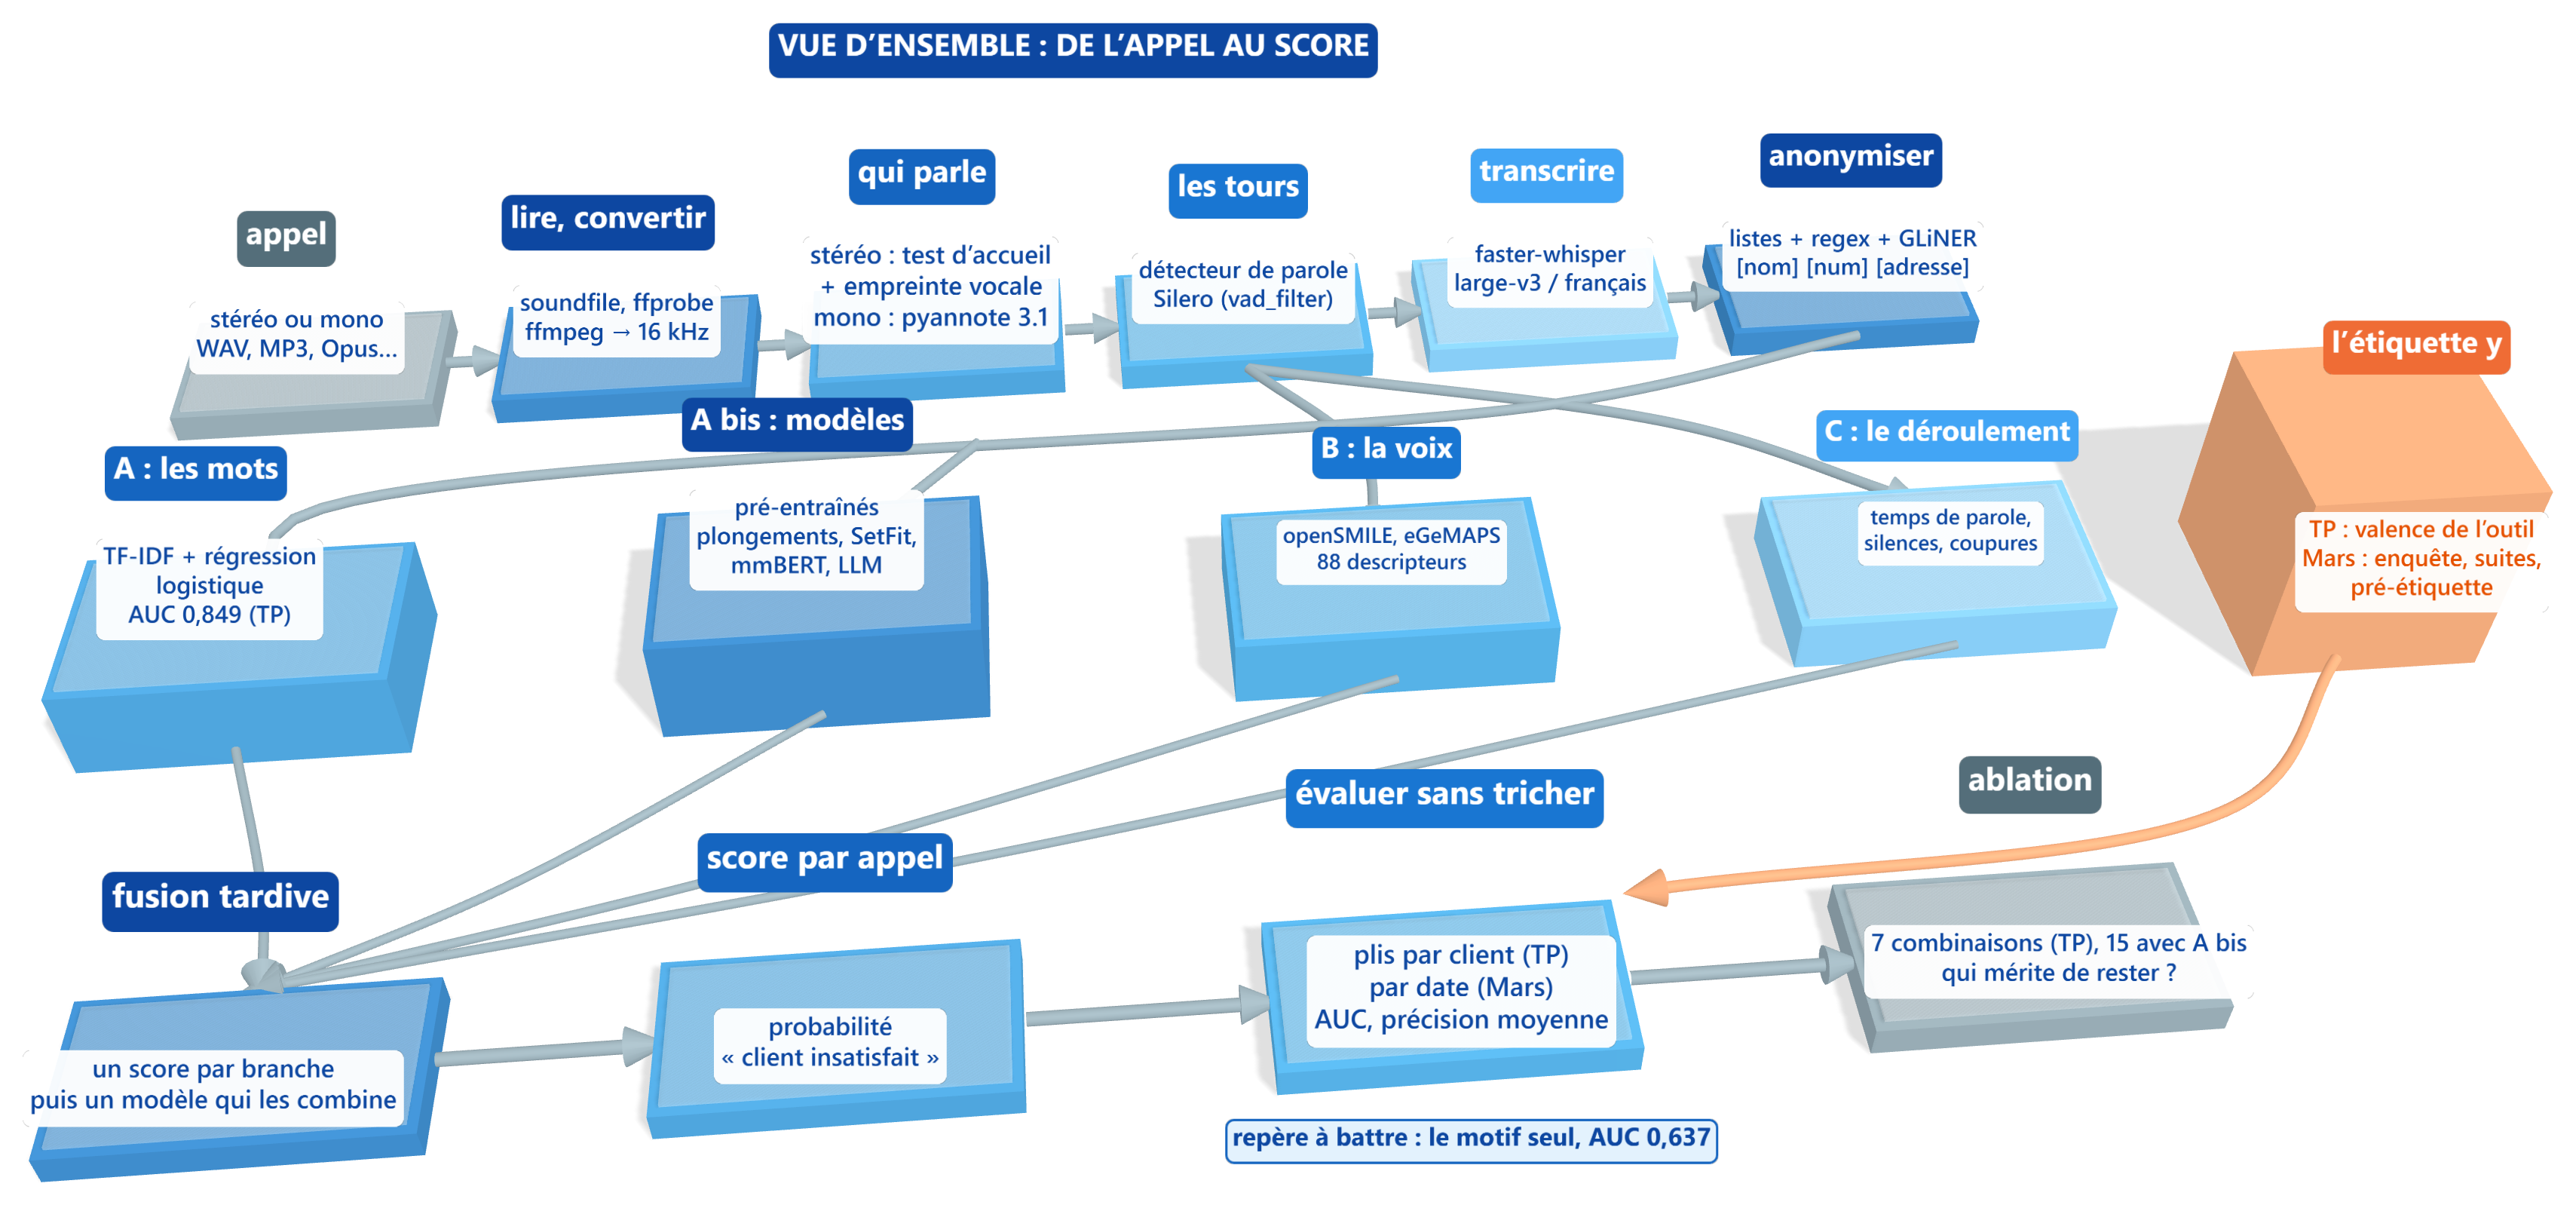
\includegraphics[width=\linewidth, height=12.2cm, keepaspectratio]{3d_ensemble.png}
\end{center}
\begin{tcbraster}[raster columns=3, raster equal height, raster column skip=6pt]
\begin{kpibox}[title={\faIcon{file-audio}\ 1. Préparer}, unbreakable]
\small Lire et convertir le son, savoir qui parle, découper les tours, transcrire, puis masquer noms et
numéros \textbf{avant tout modèle}.
\end{kpibox}
\begin{kpibox}[title={\faProjectDiagram\ 2. Des branches indépendantes}, unbreakable]
\small \textbf{A} les mots (TF-IDF), \textbf{A bis} les modèles pré-entraînés, \textbf{B} la voix,
\textbf{C} le déroulement : chacune donne un score, une fusion tardive les combine.
\end{kpibox}
\begin{kpibox}[title={\faBalanceScale\ 3. Juger honnêtement}, unbreakable]
\small Une étiquette auditée, un découpage sans tricher (par client, par date), un repère à battre
(0,637), puis l'ablation.
\end{kpibox}
\end{tcbraster}
\end{landscape}}

% Bandeau d'ouverture d'une grande partie
\newcommand{\bandeaupartie}[2]{\clearpage
\begin{tcolorbox}[colback=titlebg, colframe=titlebg, coltext=white, arc=5pt, boxrule=0pt,
  left=15pt, right=15pt, top=12pt, bottom=12pt]
\begin{center}{\Large\bfseries #1}\\[6pt]{\normalsize #2}\end{center}
\end{tcolorbox}}

\setlist[itemize]{leftmargin=1.5em, label={\color{sectioncolor}\textbullet}}
\setlist[enumerate]{leftmargin=1.5em, label={\color{sectioncolor}\arabic*.}}

% Page de titre commune : #1 sur-titre, #2 titre, #3 sous-titre, #4 ligne bleue, #5 objectif
\newcommand{\pagedetitre}[5]{%
\thispagestyle{empty}
\begin{tikzpicture}[remember picture, overlay]
  \fill[titlebg] (current page.north west) rectangle ([yshift=-8cm]current page.north east);
  \fill[lightblue] ([yshift=-8cm]current page.north west) rectangle ([yshift=-8.3cm]current page.north east);
  \fill[titlebg] (current page.south west) rectangle ([yshift=1.5cm]current page.south east);
  \fill[lightblue] ([yshift=1.5cm]current page.south west) rectangle ([yshift=1.8cm]current page.south east);
\end{tikzpicture}
\vspace*{0.1cm}
\begin{center}
  {\color{skyblue}\large\textbf{#1}}\\[0.5cm]
  {\color{white}\Huge\textbf{#2}}\\[0.4cm]
  {\color{palblue}\LARGE #3}\\[0.3cm]
  {\color{skyblue}\large #4}
\end{center}
\vspace*{1.6cm}
\begin{center}\couverture\end{center}
\vspace*{0.8cm}
\begin{center}
  \begin{tikzpicture}
    \node[fill=notebg, rounded corners=6pt, inner sep=14pt, text width=13cm, align=center,
      draw=sectioncolor, line width=0.8pt] {{\color{darkblue}\large\textbf{Objectif :} #5}};
  \end{tikzpicture}
\end{center}
\vfill
\begin{center}{\color{white}\small Année 2026--2027}\end{center}
\newpage
\setcounter{page}{1}}

% Illustration de couverture : le pipeline 1 en trois branches
\newcommand{\couverture}{%
\begin{tikzpicture}[
  b/.style={draw=##1, fill=##1!12, rounded corners=4pt, minimum width=3cm, minimum height=1.1cm,
    align=center, font=\small},
  a/.style={-{Stealth[length=2.5mm]}, thick, color=slate}]
\node[b=slate] (in) {{\Large\faPhone}\\Appel};
\node[b=darkblue, right=0.9cm of in] (d) {{\Large\faUsers}\\Qui parle ?};
\node[b=sectioncolor, right=0.9cm of d, yshift=1.5cm] (A) {{\Large\faFont}\\A : les mots};
\node[b=accentblue, right=0.9cm of d] (B) {{\Large\faWaveSquare}\\B : la voix};
\node[b=lightblue, right=0.9cm of d, yshift=-1.5cm] (C) {{\Large\faStopwatch}\\C : le rythme};
\node[b=darkblue, right=0.9cm of B] (out) {{\Large\faSmile\ \faFrown}\\Satisfait ?};
\draw[a] (in) -- (d); \foreach \x in {A,B,C} {\draw[a] (d) -- (\x); \draw[a] (\x) -- (out);}
\end{tikzpicture}}

\setlength{\parindent}{0pt}

% card : grande carte de comparaison ; bloc : encadré d'étape (style stepbox de la référence)
\newtcolorbox{card}[2]{colback=white, colframe=#1, coltitle=white, colbacktitle=#1,
  fonttitle=\bfseries\large, title={#2}, arc=3pt, boxrule=1pt, equal height group=cards,
  before upper=\raggedright}
\newtcolorbox{bloc}[2][sectioncolor]{colback=white, colframe=#1, coltitle=white,
  colbacktitle=#1, fonttitle=\bfseries, title={#2}, arc=3pt, boxrule=0.8pt,
  left=8pt, right=8pt, top=6pt, bottom=6pt}

\newcommand{\chiffre}[1]{{\Large\bfseries\color{darkblue} #1}}

\begin{document}

\pagedetitre{École d'automne IA, Alsace Tech}{Hackathon voix du client}
  {Fiches 1 à 4}{Ton GPU gratuit, puis les séances 1 à 3 du TP}
  {allumer un GPU gratuit sans gaspiller ton quota, puis vérifier tes données avant d'entraîner quoi que ce soit.}

\vuedensemble

\section{Ton GPU gratuit en ligne}

\begin{tcolorbox}[colback=notebg,colframe=sectioncolor,arc=3pt,halign=center,boxrule=1.5pt]
{\LARGE\faServer\quad\bfseries On travaille sur \textcolor{sectioncolor}{KAGGLE}.}\quad
{\large Colab sert seulement de secours.}
\end{tcolorbox}

\begin{tcbraster}[raster columns=2,raster equal height,raster column skip=8pt]
\begin{card}{sectioncolor}{\faTrophy\ Kaggle}
\begin{itemize}[leftmargin=1.3em,itemsep=3pt]
\item[\faMicrochip] \chiffre{2 × T4}, 16 Go chacune
\item[\faMemory] environ \chiffre{29 Go} de RAM
\item[\faClock] \chiffre{12 h} par session
\item[\faBatteryHalf] environ \chiffre{30 h} de GPU par semaine
\item[\faPlayCircle] tourne \textbf{en arrière-plan} (\og Save \& Run All \fg)
\item[\faSave] garde tes fichiers dans \texttt{/kaggle/working}
\end{itemize}
\end{card}
\begin{card}{slate}{\faLifeRing\ Colab gratuit (secours)}
\begin{itemize}[leftmargin=1.3em,itemsep=3pt]
\item[\faMicrochip] \chiffre{1 × T4}, 16 Go, \textbf{pas garantie}
\item[\faMemory] environ \chiffre{12,7 Go} de RAM
\item[\faClock] \chiffre{12 h} au plus, souvent moins
\item[\faQuestionCircle] quota \textbf{inconnu}, il change
\item[\faEye] l'onglet doit \textbf{rester ouvert}
\item[\faTrash] fichiers \textbf{perdus} sans copie vers Drive
\end{itemize}
\end{card}
\end{tcbraster}

\vspace{4pt}
\begin{bloc}[darkblue]{\faCalendarCheck\quad À faire AVANT le hackathon}
\begin{tikzpicture}[
  etape/.style={draw=darkblue,fill=white,rounded corners=4pt,minimum width=3.6cm,minimum height=1.5cm,
    align=center,font=\small,text width=3.4cm},
  arr/.style={-{Stealth[length=3mm]},very thick,color=darkblue}]
\node[etape] (a) {{\Large\faUserPlus}\\Créer un compte\\\textbf{kaggle.com}};
\node[etape,right=0.35cm of a] (b) {{\Large\faMobile*}\\\textbf{Vérifier ton téléphone}\\(sinon : ni GPU ni Internet)};
\node[etape,right=0.35cm of b] (c) {{\Large\faKey}\\Compte \textbf{Hugging Face}\\+ jeton de lecture};
\node[etape,right=0.35cm of c] (d) {{\Large\faCheckSquare}\\Accepter les conditions\\du modèle de \textbf{diarisation}};
\draw[arr] (a) -- (b); \draw[arr] (b) -- (c); \draw[arr] (c) -- (d);
\end{tikzpicture}
\end{bloc}

\vspace{2pt}
\begin{bloc}{\faPowerOff\quad Allumer le GPU, en 4 clics}
\begin{tikzpicture}[
  num/.style={circle,fill=sectioncolor,text=white,font=\bfseries\Large,minimum size=0.9cm},
  lab/.style={align=center,font=\small,text width=3.6cm},
  arr/.style={-{Stealth[length=3mm]},very thick,color=sectioncolor}]
\node[num] (n1) {1};
\node[num,right=3.0cm of n1] (n2) {2};
\node[num,right=3.0cm of n2] (n3) {3};
\node[num,right=3.0cm of n3] (n4) {4};
\node[lab,below=2pt of n1] {\textbf{Create} \faArrowRight\ \textbf{New Notebook}};
\node[lab,below=2pt of n2] {Panneau de droite :\\\textbf{Session options}};
\node[lab,below=2pt of n3] {\textbf{Accelerator}\\\faArrowRight\ \textbf{GPU T4 x2}};
\node[lab,below=2pt of n4] {\textbf{Internet}\\\faToggleOn\ \textbf{On}};
\draw[arr] (n1) -- (n2); \draw[arr] (n2) -- (n3); \draw[arr] (n3) -- (n4);
\end{tikzpicture}
\end{bloc}

\vspace{2pt}
\begin{bloc}[accentblue]{\faTerminal\quad Ta première cellule : vérifie ta machine}
\begin{minipage}[t]{0.55\linewidth}
\begin{lstlisting}
!nvidia-smi
!free -h
import torch
print(torch.cuda.device_count())
print(torch.cuda.get_device_name(0))
\end{lstlisting}
\end{minipage}\hfill
\begin{minipage}[t]{0.42\linewidth}
\vspace{2pt}
\textbf{\textcolor{accentblue}{\faCheckCircle\ Tu dois voir :}}
\begin{itemize}[leftmargin=1.2em,itemsep=1pt]
\item deux lignes \texttt{Tesla T4}
\item \texttt{2}
\item \texttt{Tesla T4}
\end{itemize}
\textbf{\textcolor{sectioncolor}{\faTimesCircle\ Tu vois \texttt{0} ?}}\\
Reprends l'étape 3, puis vérifie ton téléphone.
\end{minipage}
\end{bloc}

\newpage
%%%%%%%%%%%%%%%%%%%%%%%%%%%%%%%%%%%%%%%%%%%%%%%%%%%%%%%% PAGE 2
\section{Les 5 règles d'or du GPU}

\begin{tikzpicture}[
  rule/.style={draw=#1,fill=#1!10,rounded corners=5pt,minimum height=2.1cm,
    text width=7.55cm,align=left,font=\normalsize,inner sep=8pt},
  ico/.style={font=\Huge,color=#1}]
\node[rule=sectioncolor] (r1) at (0,0) {\hspace{1.4cm}\parbox{5.95cm}{\textbf{Transcris UNE fois.}\\
  Sauvegarde le résultat, puis travaille toujours sur les fichiers sauvegardés.}};
\node[ico=sectioncolor] at ($(r1.west)+(0.8,0)$) {\faSave};
\node[rule=lightblue,right=0.3cm of r1] (r2) {\hspace{1.4cm}\parbox{5.95cm}{\textbf{Arrête ta session.}\\
  Une session ouverte mange ton quota, même si rien ne tourne.}};
\node[ico=lightblue] at ($(r2.west)+(0.8,0)$) {\faStopCircle};
\node[rule=darkblue,below=0.3cm of r1] (r3) {\hspace{1.4cm}\parbox{5.95cm}{\textbf{Calcul long ?}\\
  \og Save \& Run All \fg{} : ça tourne seul, tu peux fermer l'onglet.}};
\node[ico=darkblue] at ($(r3.west)+(0.8,0)$) {\faRocket};
\node[rule=accentblue,below=0.3cm of r2] (r4) {\hspace{1.4cm}\parbox{5.95cm}{\textbf{T4 = \texttt{fp16}.}\\
  Jamais \texttt{bf16}, jamais FlashAttention.}};
\node[ico=accentblue] at ($(r4.west)+(0.8,0)$) {\faThermometerHalf};
\node[rule=slate,below=0.3cm of r3,text width=15.96cm,xshift=4.2cm] (r5)
  {\hspace{1.4cm}\parbox{13.9cm}{\textbf{2 × T4 = deux cartes de 16 Go, PAS une carte de 32 Go.}\\
  Pour aller deux fois plus vite : coupe ta liste d'appels en deux, un processus par carte (code ci-dessous).}};
\node[ico=slate] at ($(r5.west)+(0.8,0)$) {\faCopy};
\end{tikzpicture}

\vspace{8pt}
\begin{bloc}{\faCode\quad Utiliser les deux GPU : un processus par carte}
\begin{lstlisting}
import subprocess, os
procs = []
for gpu in (0, 1):
    env = dict(os.environ, CUDA_VISIBLE_DEVICES=str(gpu))   # ce processus ne voit qu'UNE carte
    procs.append(subprocess.Popen(
        ["python", "transcrire.py", "--part", str(gpu), "--nparts", "2"], env=env))
for p in procs:
    p.wait()                                                  # on attend les deux moitiés
\end{lstlisting}
\end{bloc}

\vspace{4pt}
\begin{bloc}[sectioncolor]{\faWrench\quad Ça plante ? Cherche ton message ici}
\renewcommand{\arraystretch}{1.5}\rowcolors{2}{notebg}{white}
\begin{tabularx}{\linewidth}{>{\ttfamily\small}p{5.8cm}X}
\rowcolor{titlebg}\color{white}\textbf{\normalfont Tu vois\ldots} & \color{white}\textbf{Tu fais\ldots} \\
device\_count() == 0 & \faArrowRight\ Accelerator : GPU T4 x2. Téléphone vérifié ? \\
pip : erreur réseau & \faArrowRight\ Session options : Internet \faToggleOn\ On \\
CUDA out of memory & \faArrowRight\ \texttt{batch\_size=4} \\
bfloat16 / bf16 & \faArrowRight\ remplace par \texttt{fp16=True} \\
flash\_attn / flash\_attention\_2 & \faArrowRight\ supprime l'option \texttt{attn\_implementation} \\
diarisation : 401 / gated / token & \faArrowRight\ jeton Hugging Face + conditions acceptées sur la page du modèle \\
quota épuisé & \faArrowRight\ un coéquipier lance le calcul depuis son compte \\
\end{tabularx}
\end{bloc}

\vfill
\begin{center}\color{slate}\small
\faUserTie\quad Une question ? Lève la main, l'encadrante passe.
\end{center}

% Copyright (c) 2026 Selina Cheggour. Tous droits réservés. Voir le fichier LICENSE.
% Fiche 2 : séance 1 du TP (parties 0 à 3). Visuelle, sans explications longues : l'encadrante explique à l'oral.
% Les valeurs « Tu dois voir » sont celles des cellules de vérification du notebook.

\newcommand{\doisvoir}[1]{\par\smallskip{\color{accentblue}\faCheckCircle\ \textbf{Tu dois voir :}} #1}
\newcommand{\image}[1]{\par\smallskip{\color{lightblue}\faChild}\ \textit{#1}}

\bandeaupartie{Fiche 2 : séance 1}{Avant d'entraîner quoi que ce soit, on vérifie.}

\section{La séance en une image}

\begin{center}
\begin{tikzpicture}[
  etape/.style={draw=#1, fill=#1!10, rounded corners=6pt, minimum width=3.55cm, minimum height=2.7cm,
    align=center, text width=3.3cm, font=\small},
  fl/.style={-{Stealth[length=3mm]}, very thick, color=slate}]
\node[etape=slate] (p0) {{\huge\faTools}\\[3pt]\textbf{0. Installer}\\corpus, 2 bibliothèques, outils};
\node[etape=sectioncolor, right=0.4cm of p0] (p1) {{\huge\faBoxOpen}\\[3pt]\textbf{1. Vérifier}\\les données sont-elles ce qu'on croit ?};
\node[etape=accentblue, right=0.4cm of p1] (p2) {{\huge\faTag}\\[3pt]\textbf{2. Définir}\\que prédit-on, au juste ?};
\node[etape=darkblue, right=0.4cm of p2] (p3) {{\huge\faBalanceScale}\\[3pt]\textbf{3. Mesurer}\\sans tricher};
\draw[fl] (p0) -- (p1); \draw[fl] (p1) -- (p2); \draw[fl] (p2) -- (p3);
\end{tikzpicture}
\end{center}

\begin{enfant}
\textbf{Comme une recette de gâteau} : vérifier que le sachet \og sucre \fg{} contient du sucre,
choisir quel gâteau, et décider comment on saura s'il est réussi. \emph{Avant} d'allumer le four.
\end{enfant}

\section{Partie 0 : mise en route}

\begin{stepbox}[title={\faPlay\quad Exécute les 3 cellules, sans rien modifier}]
\begin{tabularx}{\linewidth}{>{\bfseries\color{sectioncolor}}c X}
0.1 & \faDownload\ télécharge le corpus : environ 650 Mo, 3 Go sur le disque. Quelques minutes, sans affichage. \\
0.2 & \faPuzzlePiece\ installe \texttt{opensmile} (la voix) et \texttt{jiwer} (les erreurs de transcription). \\
0.3 & \faToolbox\ charge les outils du TP, dont \texttt{verifier}. \\
\end{tabularx}
\doisvoir{\texttt{1446 appels disponibles}, puis \texttt{Outils chargés.} et la liste des versions.}
\end{stepbox}

\begin{tcbraster}[raster columns=2, raster equal height, raster column skip=8pt, raster every box/.style={unbreakable}]
\begin{enfant}[unbreakable]
\texttt{/kaggle/working} = le \textbf{cartable}, pesé à chaque sauvegarde.
\texttt{/kaggle/temp} = la \textbf{table}, nettoyée le soir. Le corpus va sur la table.
\end{enfant}
\begin{enfant}[unbreakable]
\texttt{[À revoir]} = la maîtresse écrit \og à revoir \fg{} dans la marge, avec un
\textbf{indice}, au lieu de déchirer la copie. Lis l'indice !
\end{enfant}
\end{tcbraster}

\section{Partie 1 : contrôle à la réception}

\begin{center}
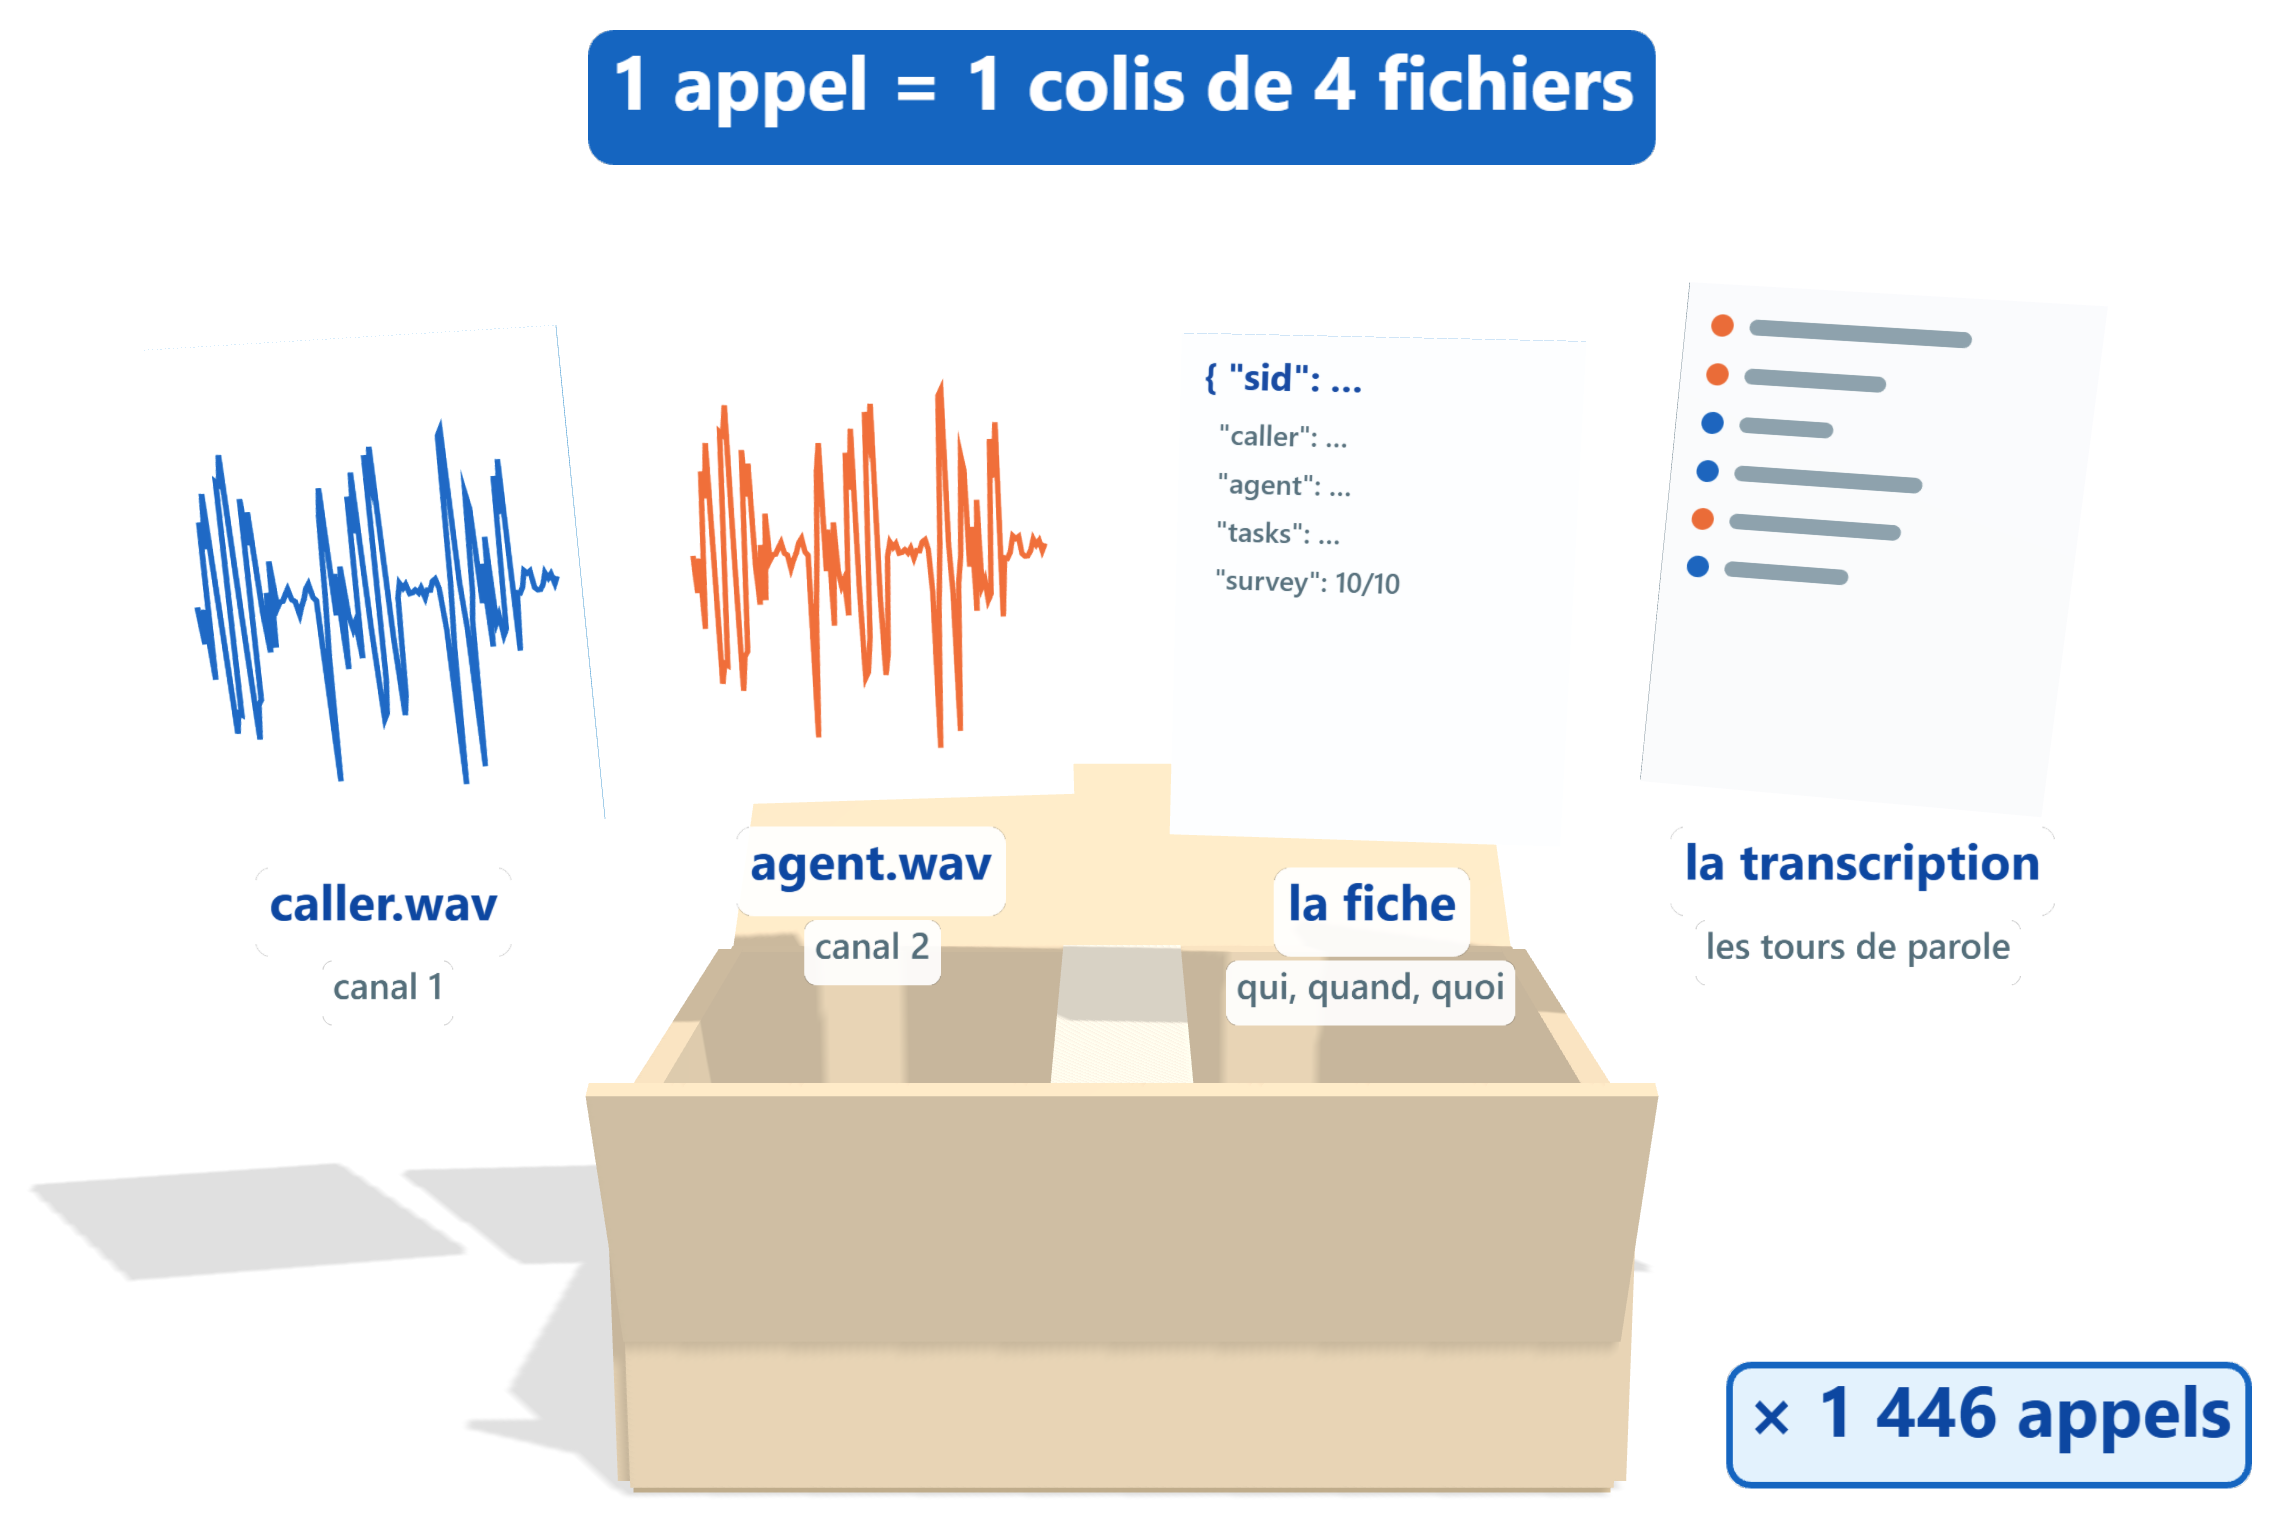
\includegraphics[width=0.68\linewidth]{3d_colis.png}
\end{center}

\begin{tcbraster}[raster columns=3, raster equal height, raster column skip=6pt, raster every box/.style={unbreakable}]
\begin{kpibox}[title={\faHeadphones\ Un canal}, unbreakable]
\small une ligne enregistrée à part : canal 1 = client, canal 2 = conseiller (en principe).
\image{deux talkies-walkies, deux cassettes}
\end{kpibox}
\begin{kpibox}[title={\faComments\ Un tour}, unbreakable]
\small un moment où une seule personne parle.
\image{chacun son tour d'avoir la balle}
\end{kpibox}
\begin{kpibox}[title={\faWind\ Un faux tour}, unbreakable]
\small un souffle ou un clic détecté comme un tour : \texttt{[noise]}.
\image{la lampe qui s'allume quand passe un chat}
\end{kpibox}
\end{tcbraster}

\begin{stepbox}[title={1.1\quad Deux tables : \texttt{appels} (1 ligne par appel) et \texttt{tours} (1 ligne par tour)}]
\doisvoir{}
\begin{center}
\cle{1\,446}{appels}\hspace{3pt}\cle{25\,730}{tours}\hspace{3pt}\cle{56 s}{médiane d'un appel}\hspace{3pt}\cle{9 s}{d'attente (médiane)}\hspace{3pt}\cle{55}{clients}
\end{center}
\end{stepbox}

\begin{stepbox}[title={1.2\quad Le client est-il toujours sur le canal 1 ?}]
Pour chaque appel : le canal le plus fréquent des tours du client. Compte ceux qui ne sont pas 1.
\doisvoir{\textbf{37 appels inversés.} Ce n'est pas ton code : c'est dans la base.}
\end{stepbox}

\begin{stepbox}[title={1.3\quad Les deux horloges : l'exercice le plus important}]
\begin{center}
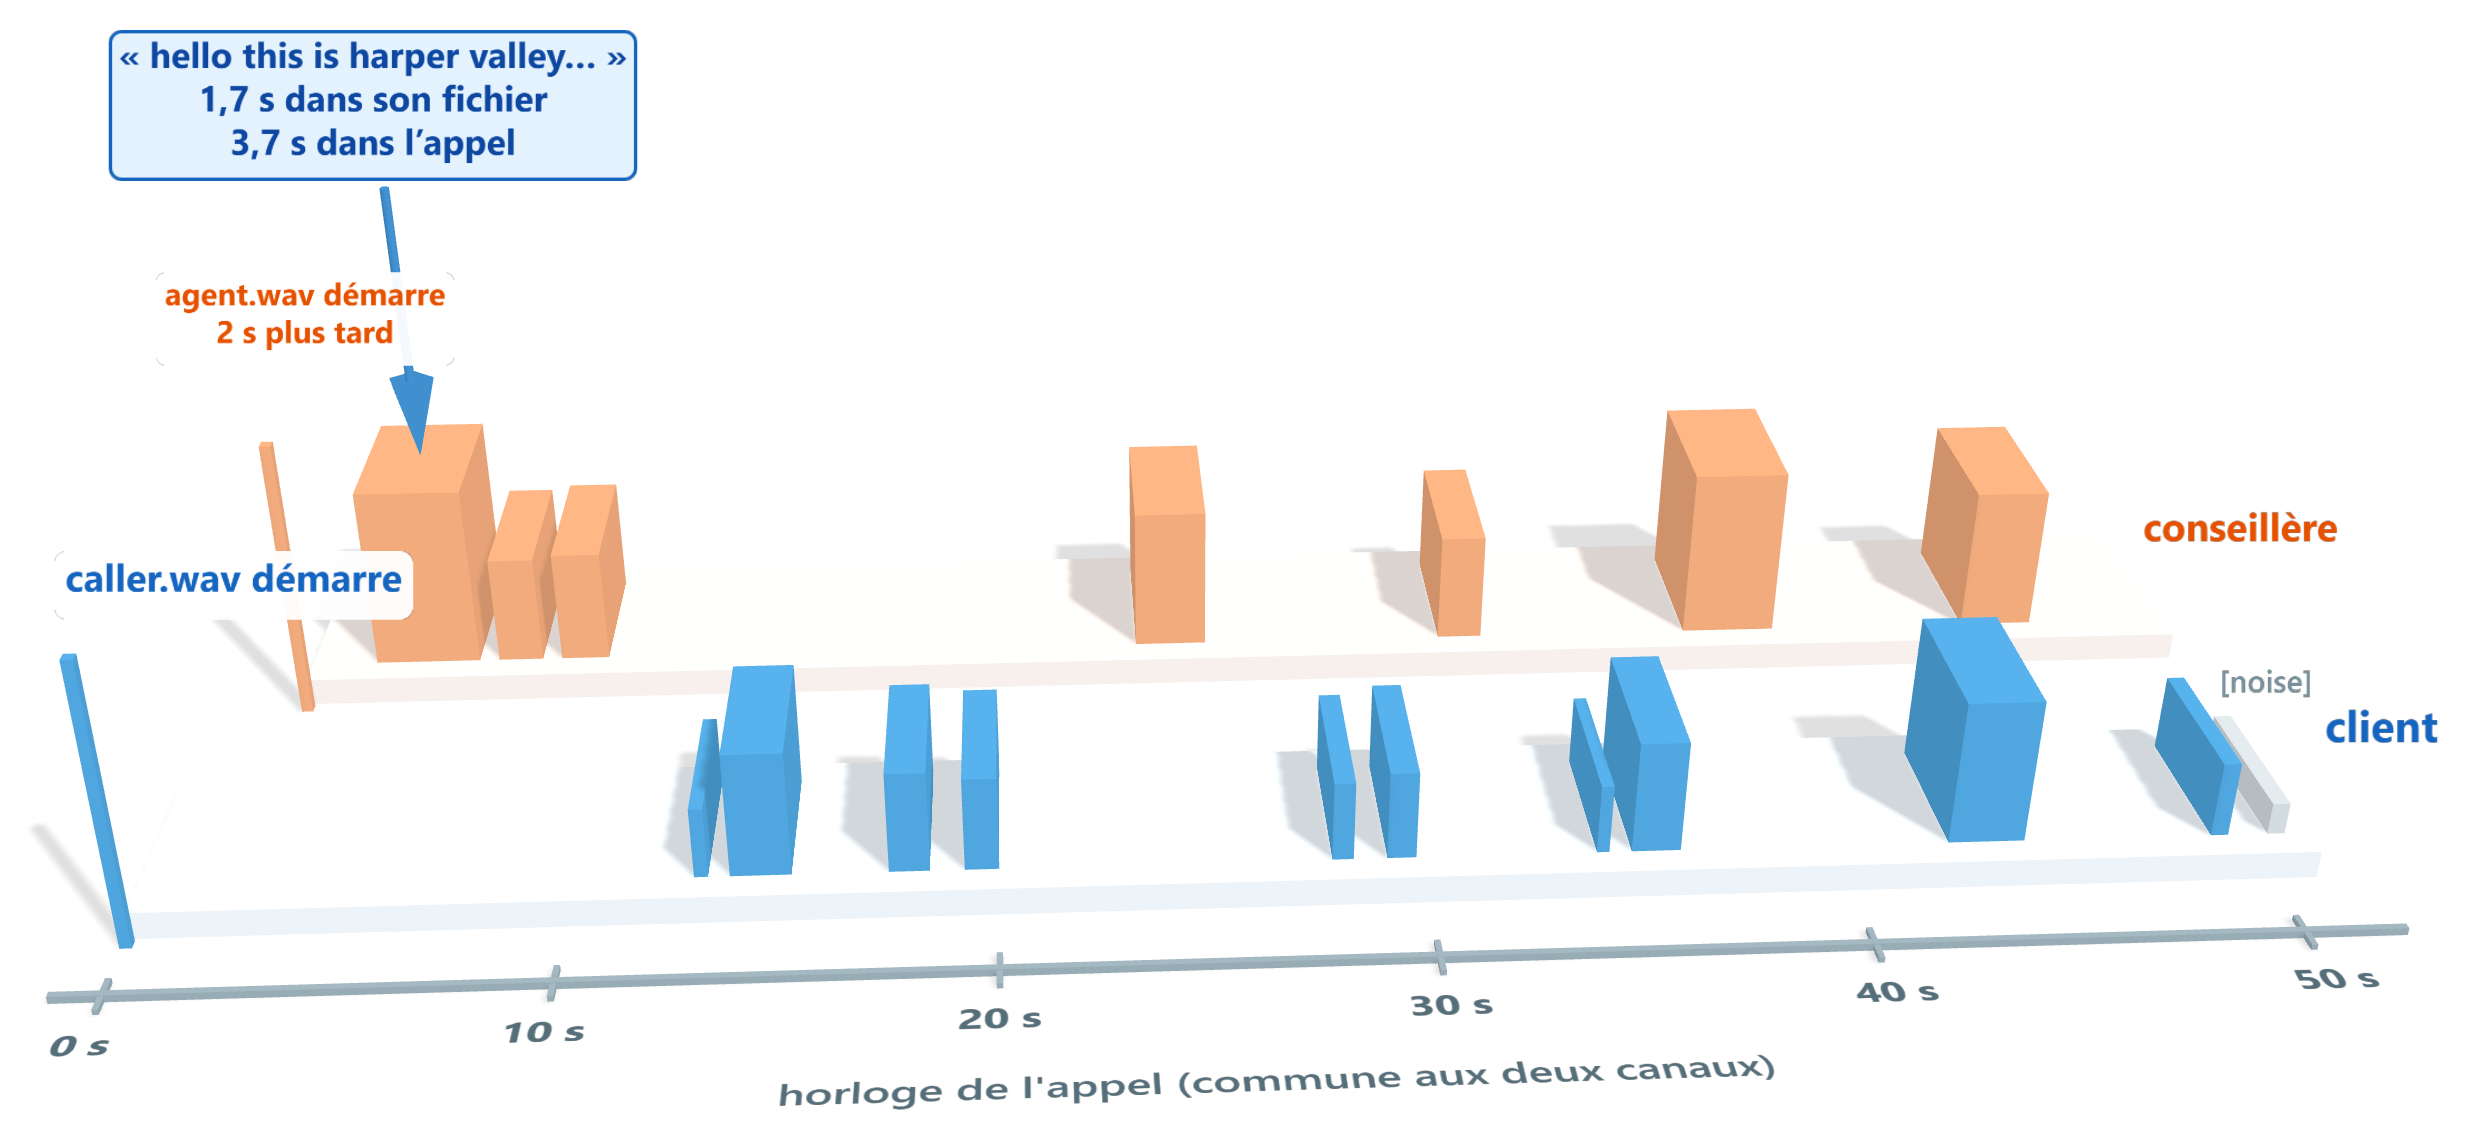
\includegraphics[width=\linewidth]{3d_pistes.png}
\end{center}
\begin{tcbraster}[raster columns=2, raster equal height, raster column skip=6pt, raster every box/.style={unbreakable}]
\begin{conceptbox}[title={\faFileAudio\ \texttt{position\_s} : où est la voix \textbf{dans son fichier}}]
pour \textbf{découper} l'audio (branche B)\\
\faArrowRight\ c'est \texttt{start\_ms}
\end{conceptbox}
\begin{conceptbox}[title={\faClock\ \texttt{debut\_s} : quand \textbf{dans l'appel}}]
pour \textbf{ordonner} les tours (branche C)\\
\faArrowRight\ c'est \texttt{offset\_ms}
\end{conceptbox}
\end{tcbraster}
\image{deux chronomètres : celui de la conseillère est lancé 2 secondes après celui de la cliente.}
\doisvoir{écart médian de \textbf{2,01 s} sur le canal 2, 0 sur le canal 1 ; la voix est à
\texttt{start\_s} dans \textbf{96 \%} des 1\,000 tours testés.}
\end{stepbox}

\begin{piege}
\textbf{C'est l'inverse de ce que dit la documentation.} En la croyant, tu découpes le conseiller
2~s trop tard dans 70~\% des appels, et ton code ne t'affiche \textbf{aucune erreur}.
\end{piege}

\begin{stepbox}[title={1.4\quad Dans quel fichier est la voix du client ?}]
Dans les 37 appels inversés, mesure l'énergie de chaque tour du client dans \texttt{caller} et dans
\texttt{agent}. Le fichier le plus fort contient sa voix.
\doisvoir{\textbf{162 tours testés}, \texttt{agent} plus fort dans \textbf{89 \%} des cas.}
\begin{center}
\begin{tikzpicture}[r/.style={draw=sectioncolor, fill=notebg, rounded corners=5pt, minimum height=1cm, align=center, font=\small, text width=6.6cm}]
\node[r] (a) {\textbf{Règle :} le fichier se choisit par le \textbf{canal},\\le rôle se lit dans la transcription.};
\node[right=0.4cm of a, align=left, font=\small] {\texttt{canal 1} \faArrowRight\ \texttt{caller/}\\\texttt{canal 2} \faArrowRight\ \texttt{agent/}};
\end{tikzpicture}
\end{center}
\image{deux tiroirs avec des étiquettes collées à l'envers : on ouvre et on regarde.}
\end{stepbox}

\begin{stepbox}[title={1.5\quad Regarde et écoute (rien à coder)}]
Change \texttt{sid\_exemple} (\texttt{appels.index[10]}, \texttt{[200]}\ldots) et écoute l'autre canal.
\faEye\ Toutes les zones colorées contiennent-elles de la parole ?
\end{stepbox}

\begin{stepbox}[title={1.6\quad Nettoyer et écarter le bruit}]
\texttt{nettoyer} : minuscules, sans \texttt{[balises]} ni \texttt{<unk>}, seulement lettres,
apostrophe, espaces. \texttt{parole} = la transcription \textbf{automatique} nettoyée n'est pas vide.
\doisvoir{\textbf{14,4 \%} des tours du client sans parole.}
\end{stepbox}

\section{Partie 2 : l'étiquette}

\begin{formulabox}
\centering\large $\text{valence} = p_{\text{pos}} - p_{\text{neg}}$ \qquad
\faArrowRight\qquad $y = 1$ si l'appel est dans le \textbf{quart le plus bas}
\end{formulabox}

\begin{enfant}
\textbf{Un thermomètre d'humeur, pas l'humeur.} $y=1$ ne veut pas dire \og client mécontent \fg{},
mais \og l'outil l'a trouvé moins positif que les autres \fg{}.
\end{enfant}

\begin{stepbox}[title={2.1 à 2.4\quad Construire, puis auditer l'étiquette}]
\begin{tabularx}{\linewidth}{>{\bfseries\color{sectioncolor}}c X >{\raggedright\arraybackslash}p{4.6cm}}
2.1 & construire \texttt{valence}, \texttt{valence\_client}, \texttt{seuil}, \texttt{y} & \faCheckCircle\ seuil \textbf{0,039} ; \textbf{362} appels à 1 \\
2.2 & lire les 15 tours les plus négatifs et les 15 plus positifs & \faCheckCircle\ \textbf{3\,322} tours candidats \\
2.3 & part de $y=1$ par motif et par client & \faCheckCircle\ \textbf{8} motifs, \textbf{45} clients \\
2.4 & la même phrase \og hi my name is\ldots \fg{} selon le nom & \faCheckCircle\ \textbf{386} présentations \\
\end{tabularx}
\end{stepbox}

\begin{center}
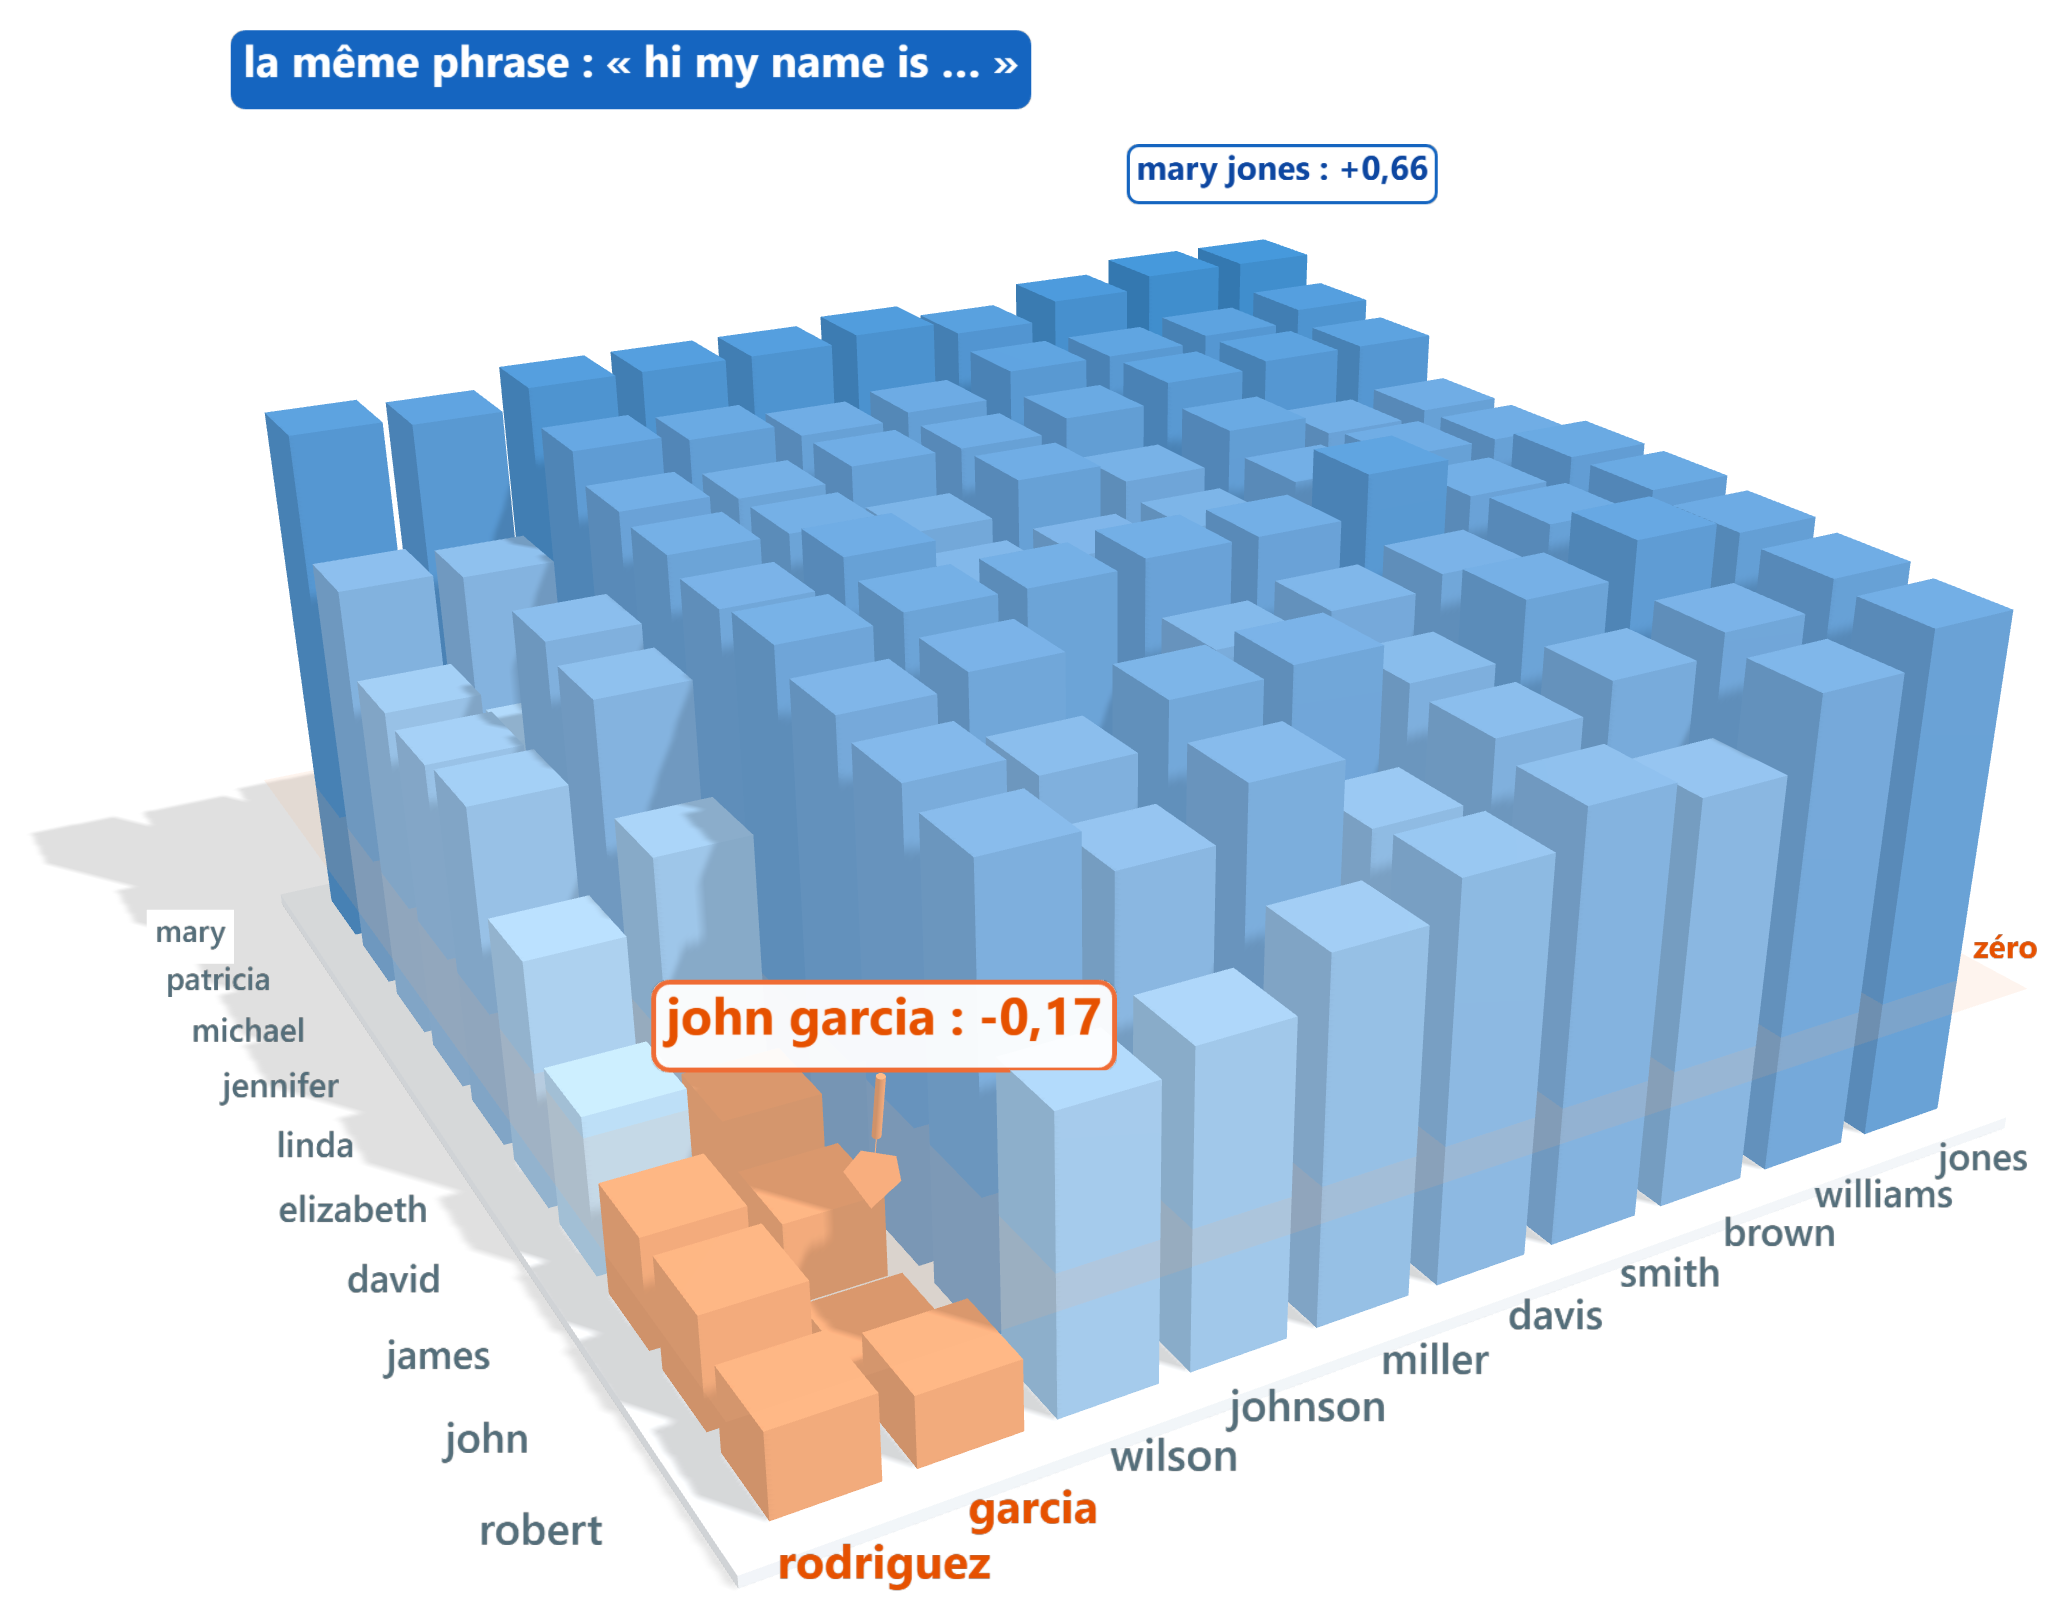
\includegraphics[width=0.66\linewidth]{3d_grille.png}
\end{center}

\begin{piege}
\textbf{La même phrase, deux notes.} \og John Garcia \fg{} : $-0{,}17$. \og Mary Jones \fg{} :
$+0{,}66$. Le nom change la note de l'outil. \faArrowRight\ On \textbf{anonymise avant} tout outil
de sentiment.\par\smallskip
\textbf{Retiens :} un nom dans le texte, même celui d'un personnage fictif, devient un biais. Dans notre
projet, on masque les noms \textbf{dès le départ} : \texttt{[nom]} pour tout le monde.
\end{piege}

\clearpage
\section{Partie 3 : mesurer sans tricher}

\begin{center}
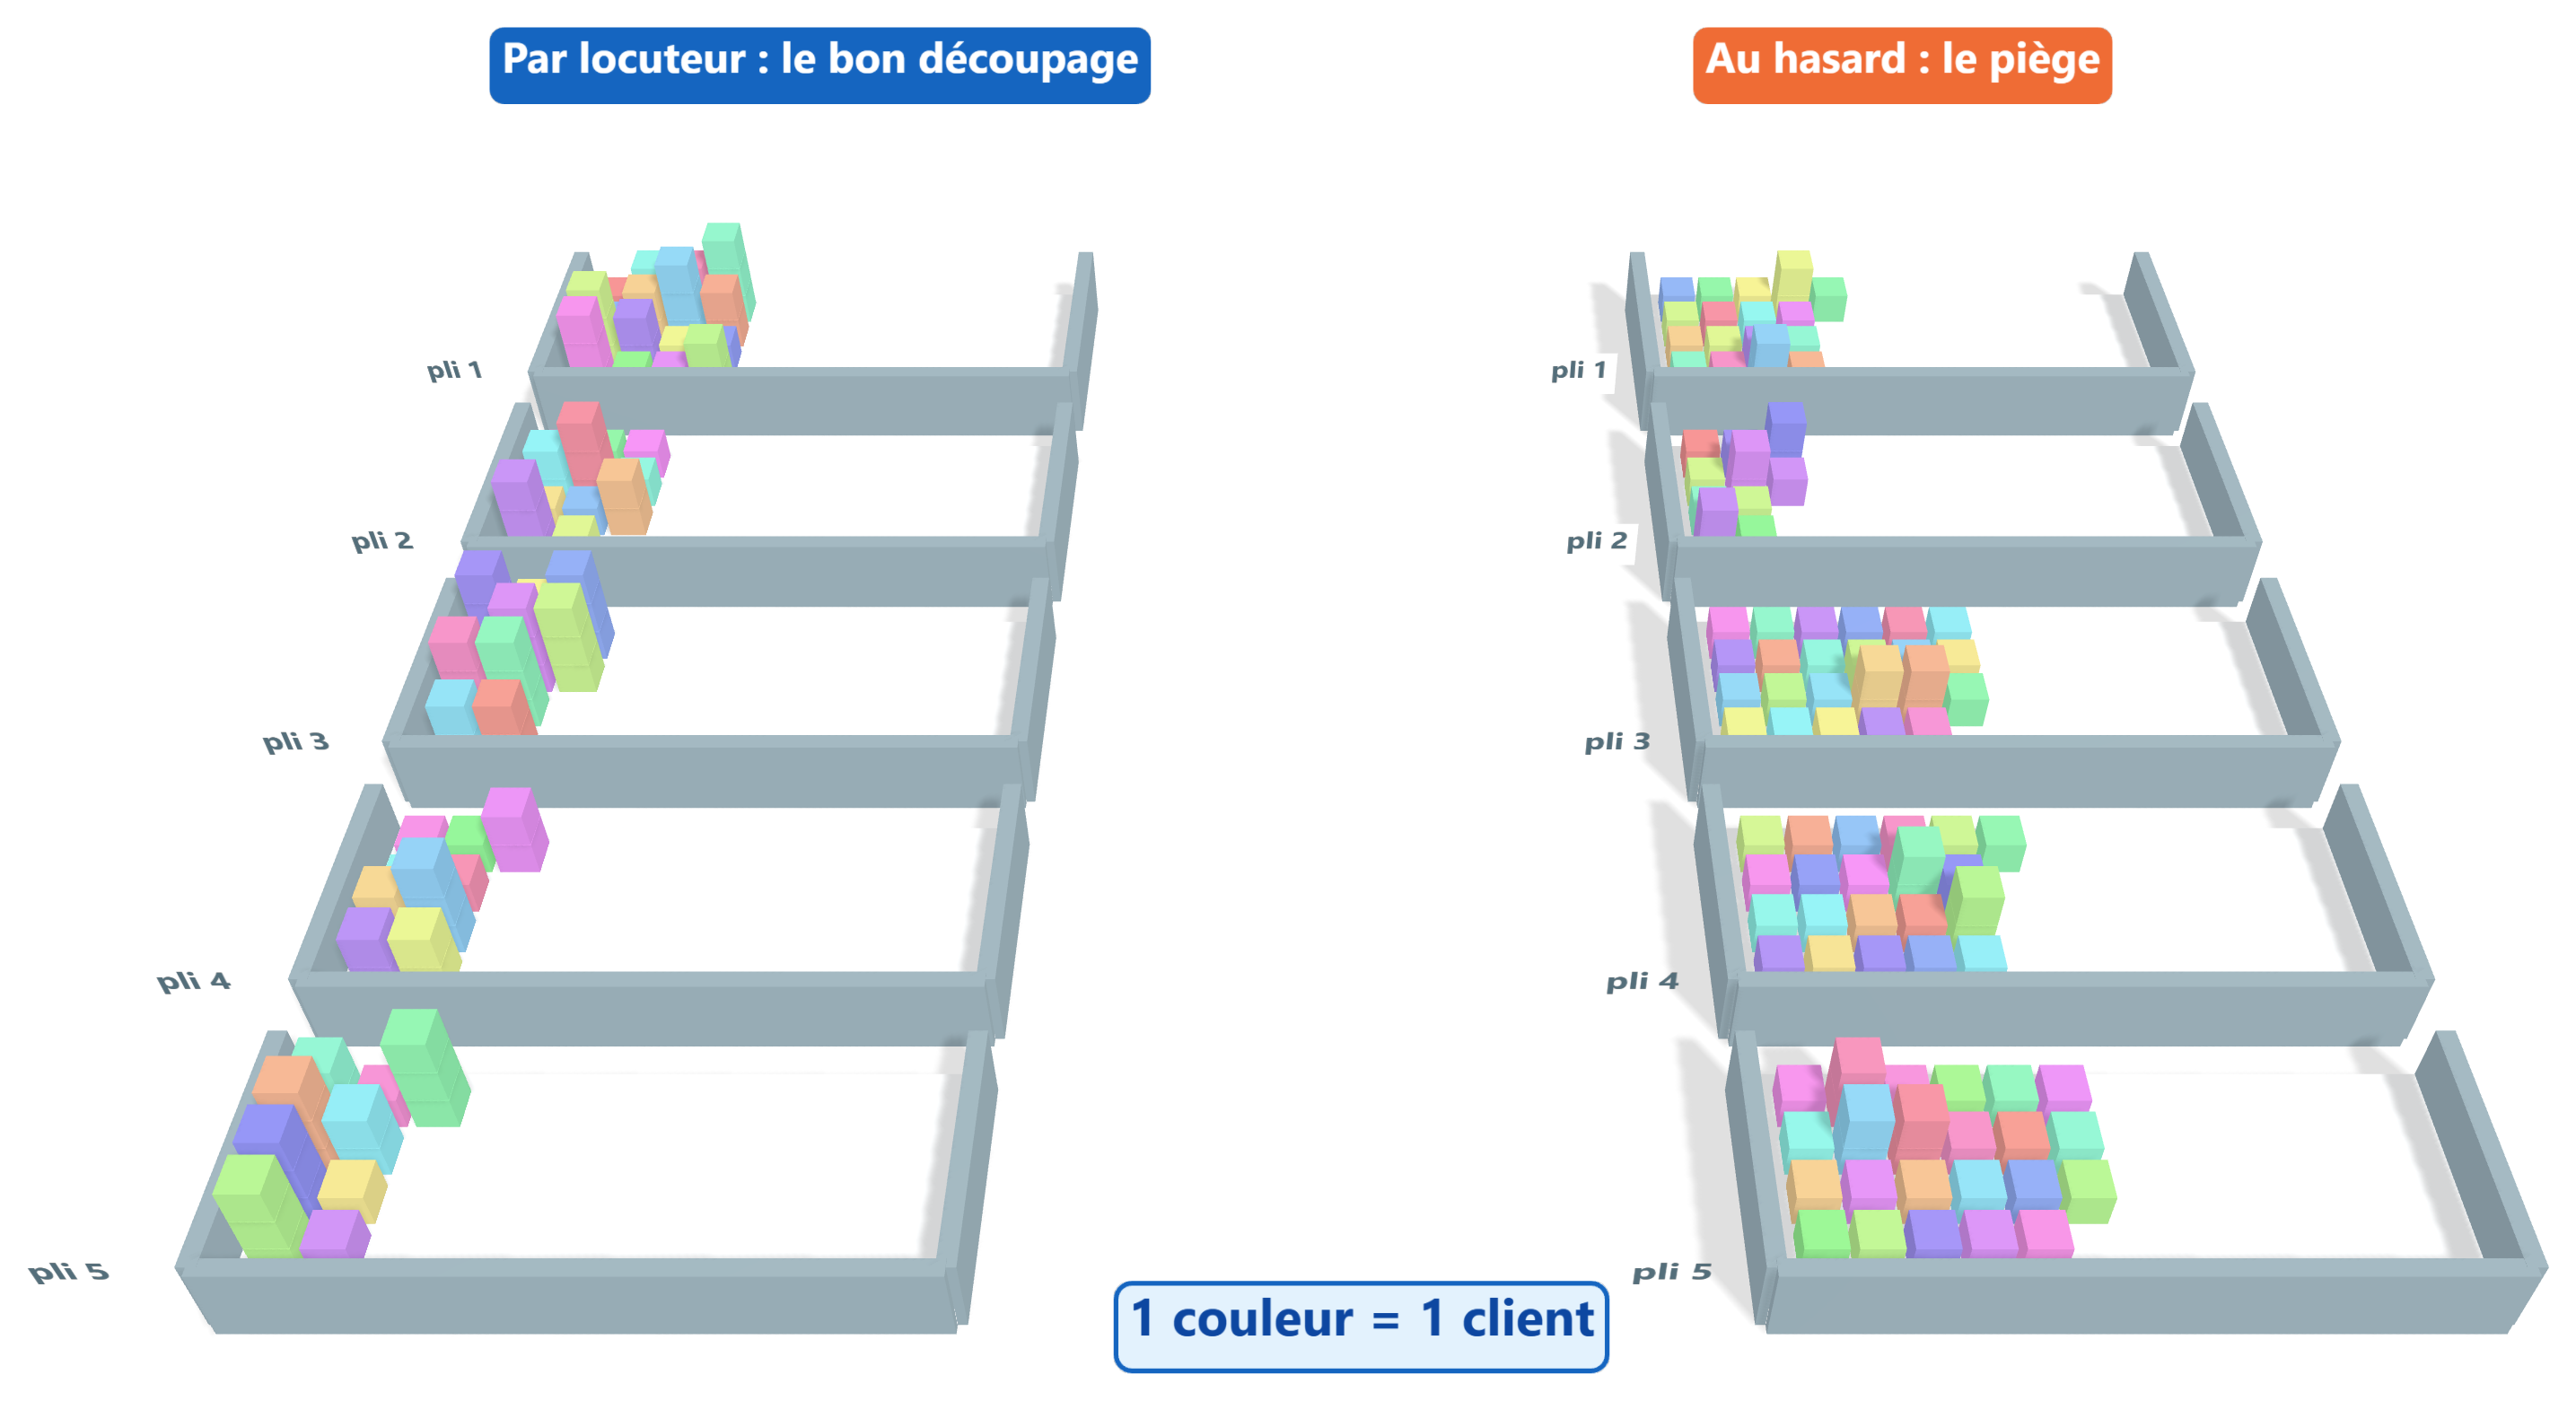
\includegraphics[width=0.92\linewidth]{3d_plis.png}
\end{center}

\begin{enfant}
\textbf{Examen et révisions} : à l'examen, pas d'exercices de la même personne qu'en révision,
sinon on reconnaît l'écriture au lieu de comprendre. Ici : \textbf{tous les appels d'un client du
même côté}.
\end{enfant}

\begin{center}
\begin{tikzpicture}[x=1.3cm, y=0.55cm]
\foreach \e in {0,...,4} {
  \node[anchor=east, font=\small] at (-0.15,-\e) {expérience \e};
  \foreach \p in {0,...,4} {
    \ifnum\p=\e
      \fill[orange!80!red] (\p,-\e-0.4) rectangle (\p+0.95,-\e+0.4);
      \node[font=\scriptsize\bfseries, color=white] at (\p+0.475,-\e) {test};
    \else
      \fill[sectioncolor!70] (\p,-\e-0.4) rectangle (\p+0.95,-\e+0.4);
    \fi
  }
}
\node[anchor=west, font=\small, text width=5.2cm] at (5.2,-2) {\faArrowRight\ chaque appel est testé \textbf{une fois}, par un modèle qui ne l'a jamais vu : ce sont les \textbf{scores hors pli}};
\end{tikzpicture}
\end{center}

\begin{stepbox}[title={3.1\quad Les plis}]
\begin{lstlisting}
plis = list(StratifiedGroupKFold(n_splits=5, shuffle=True, random_state=0)
            .split(appels, y, groups=appels.id_client))
\end{lstlisting}
\doisvoir{5 plis de \textbf{273 à 321} appels, \textbf{9 à 16} clients chacun, aucun client des deux côtés.}
\end{stepbox}

\begin{tcbraster}[raster columns=2, raster equal height, raster column skip=8pt, raster every box/.style={unbreakable}]
\begin{kpibox}[title={\faTrophy\ AUC}, unbreakable]
On tire un appel à 1 et un appel à 0 : chance que le modèle classe le 1 plus haut.\\
\textbf{0,5} = pile ou face \quad \textbf{1} = parfait
\image{le jeu des deux enveloppes}
\end{kpibox}
\begin{kpibox}[title={\faListOl\ Précision moyenne}, unbreakable]
Regarde surtout le \textbf{haut de la liste} : les appels qu'on remonterait à un superviseur.\\
\textbf{0,25} = hasard
\end{kpibox}
\end{tcbraster}

\begin{stepbox}[title={3.2\quad Le repère à battre : le motif seul}]
\doisvoir{}
\begin{center}
\cle{0,637}{AUC}\hspace{8pt}\cle{0,349}{précision moyenne}
\end{center}
\end{stepbox}

\begin{piege}[unbreakable]
\textbf{Ta barre, c'est 0,637, pas 0,5.} Une branche à 0,62 n'a rien appris : le motif seul fait
mieux.
\image{deviner la météo en disant \og comme aujourd'hui \fg{} : le vrai météorologue doit faire mieux.}
\end{piege}

\begin{conceptbox}[title={La barre \og motif seul \fg{} que tu verras avant la branche A}, unbreakable]
\small Ce n'est pas une branche. C'est un modèle qui ne connaît que la raison de l'appel (\og pay bill \fg{},
\og get branch hours \fg{}\ldots), recalculé dans les mêmes plis et posé à côté des branches pour servir
de ligne de lecture. Il atteint 0,637 parce que certains motifs sont plus pénibles que d'autres : 47\,\%
d'appels étiquetés~1 pour \og pay bill \fg{}, 11\,\% pour \og get branch hours \fg{}.
\begin{center}
\begin{tikzpicture}[x=26cm, y=1cm, font=\footnotesize]
\fill[slate!12] (0.45,-0.35) rectangle (0.637,0.35);
\fill[notebg] (0.637,-0.35) rectangle (0.91,0.35);
\draw[thick, ->] (0.45,0) -- (0.915,0) node[right] {AUC};
\foreach \v/\l in {0.5/0{,}5, 0.6/0{,}6, 0.7/0{,}7, 0.8/0{,}8, 0.9/0{,}9} \draw (\v,-0.07) -- (\v,0.07) node[pos=0, below=8pt] {\l};
\draw[very thick, darkblue] (0.637,-0.65) -- (0.637,0.65) node[pos=0, below=2pt, font=\footnotesize\bfseries] {motif seul 0,637};
\foreach \v/\n/\c in {0.526/{B, 0,526}/sectioncolor, 0.614/{C, 0,614}/slate, 0.849/{A, 0,849}/accentblue}
  \fill[\c] (\v,0) circle (2.8pt) node[above=6pt, font=\footnotesize\bfseries, color=\c] {\n};
\end{tikzpicture}
\end{center}
À gauche de la ligne : la branche n'a rien appris de plus que le motif. À droite : elle apporte de
l'information sur la tonalité.
\end{conceptbox}

\begin{tcolorbox}[colback=titlebg, colframe=titlebg, coltext=white, arc=5pt, boxrule=0pt,
  left=15pt, right=15pt, top=10pt, bottom=10pt]
\begin{center}
{\Large\bfseries En fin de séance, tu as :}\\[8pt]
\begin{tabular}{c c c}
{\huge\faTable} & {\huge\faTag} & {\huge\faBalanceScale} \\[4pt]
\textbf{2 tables propres} & \textbf{1 étiquette} & \textbf{1 protocole} \\
\texttt{appels}, \texttt{tours} & dont tu connais les défauts & plis par client, repère 0,637 \\
\end{tabular}
\end{center}
\end{tcolorbox}

% Fiche 3 : séance 2 du TP (partie 4, les mots). Commencée le 17/10/2026 avec l'exercice 4.3 ;
% les exercices 4.1, 4.2, 4.4 et 4.5 viendront ensuite.

\bandeaupartie{Fiche 3 : séance 2}{Les mots : ton premier classifieur.}

\section{Deux modèles, les mêmes briques}

\begin{center}
\begin{tikzpicture}[
  b/.style={draw=#1, fill=#1!10, rounded corners=6pt, text width=3.1cm, align=center, font=\small,
    minimum height=1.8cm, inner sep=4pt},
  fl/.style={-{Stealth[length=2.5mm]}, very thick, color=slate}]
\node[b=slate] (m) {{\Large\faTag}\\\textbf{le motif}};
\node[b=sectioncolor, right=0.5cm of m] (o) {\texttt{OneHotEncoder}\\une case par motif};
\node[b=darkblue, right=0.5cm of o] (l) {\texttt{\footnotesize LogisticRegression}\\un poids par case};
\node[b=accentblue, right=0.5cm of l] (r) {\textbf{3.2 : repère}\\AUC \textbf{0,637}};
\draw[fl] (m) -- (o); \draw[fl] (o) -- (l); \draw[fl] (l) -- (r);
\node[b=slate, below=0.5cm of m] (t) {{\Large\faComment}\\\textbf{les mots du client}};
\node[b=sectioncolor, right=0.5cm of t] (v) {\texttt{TfidfVectorizer}\\une colonne par mot};
\node[b=darkblue, right=0.5cm of v] (l2) {\texttt{\footnotesize LogisticRegression}\\un poids par mot};
\node[b=accentblue, right=0.5cm of l2] (r2) {\textbf{4.3 : branche A}\\AUC \textbf{0,86}};
\draw[fl] (t) -- (v); \draw[fl] (v) -- (l2); \draw[fl] (l2) -- (r2);
\end{tikzpicture}
\end{center}

\begin{tcbraster}[raster columns=2, raster equal height, raster column skip=8pt]
\begin{enfant}[unbreakable]
\texttt{OneHotEncoder} : \textbf{une case cochée par motif}, comme sur un formulaire. Un modèle ne
sait pas lire \og pay bill \fg{}, il sait lire des 0 et des 1.
\end{enfant}
\begin{enfant}[unbreakable]
\texttt{LogisticRegression} : \textbf{une balance à mots}. Chaque mot pose un petit poids d'un côté ou
de l'autre ; la balance penche, et on lit un pourcentage entre 0 et 100.
\end{enfant}
\end{tcbraster}

\section{TF-IDF : un appel devient une ligne de nombres}

\begin{center}
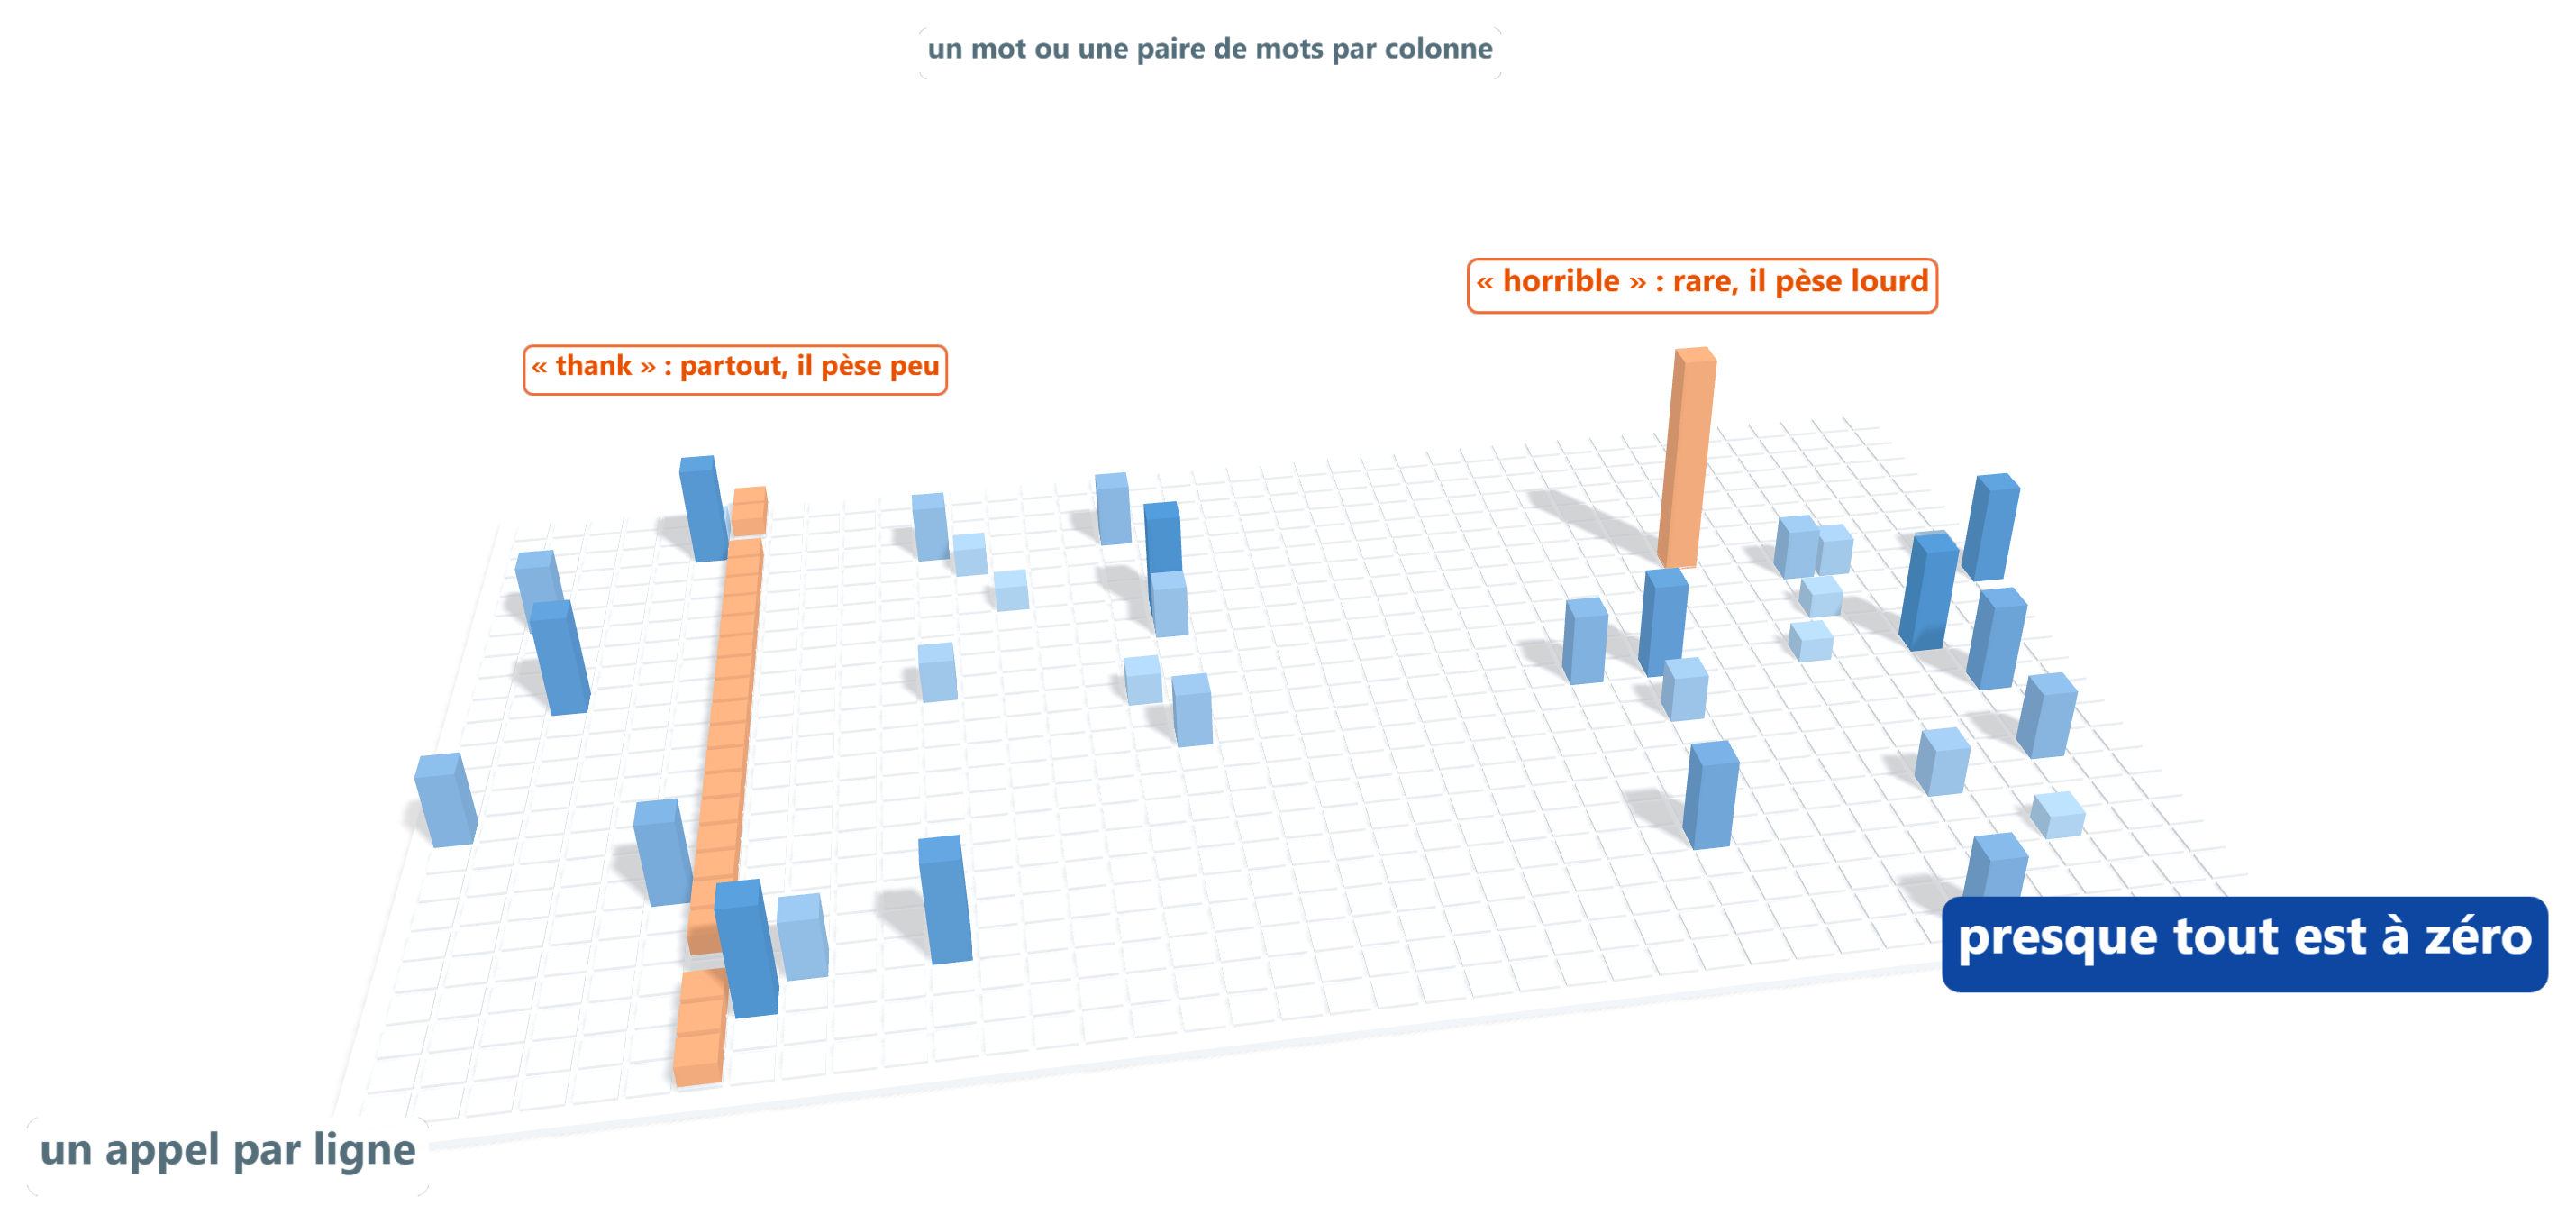
\includegraphics[width=0.8\linewidth]{3d_tfidf.png}
\end{center}

\begin{formulabox}
\centering\large TF-IDF $=$ \textbf{TF} {\small (le mot est-il \emph{ici} ?)} $\times$ \textbf{IDF} {\small (est-il \emph{rare} ailleurs ?)}
\end{formulabox}

\begin{center}
\begin{tikzpicture}[x=1.35cm, y=0.55cm]
\foreach \m/\n/\v [count=\i from 0] in {my/1\,422/1.02, thank/1\,040/1.33, bye/413/2.25, address/252/2.74, card/189/3.03, appreciate/8/6.08} {
  \pgfmathsetmacro{\c}{\v/6.08*100}
  \fill[sectioncolor!\c!skyblue] (0,-\i-0.35) rectangle (\v,-\i+0.35);
  \node[anchor=east, font=\small\ttfamily] at (-0.1,-\i) {\m};
  \node[anchor=west, font=\small] at (\v+0.08,-\i) {\textbf{\v} {\color{slate}\footnotesize dans \n{} appels}};
}
\node[font=\small\bfseries, color=darkblue] at (3,1.0) {IDF sur les 1\,446 appels du TP : plus rare = plus lourd};
\end{tikzpicture}
\end{center}

\begin{tcbraster}[raster columns=2, raster equal height, raster column skip=8pt]
\begin{enfant}[unbreakable]
\textbf{Un sac de mots} : on vide la phrase dans un sac et on compte, en donnant plus de poids aux mots
rares. Le sac sait que \og horrible \fg{} est dedans, pas qu'on a dit \og pas horrible \fg{}.
\end{enfant}
\begin{kpibox}[title={\faCalculator\ Dans ton TP}, unbreakable]
\small \textbf{2\,220} colonnes, \textbf{97,7\,\%} de zéros, \textbf{47} mots allumés par appel. Le
premier appel ressort avec \og debit card \fg{} : le TF-IDF a trouvé seul de quoi il parle.
\end{kpibox}
\end{tcbraster}

\begin{tcbraster}[raster columns=3, raster equal height, raster column skip=6pt]
\begin{kpibox}[title={\texttt{ngram\_range=(1, 2)}}, unbreakable]
\small mots seuls \textbf{et} paires de mots : \og thank \fg{} et \og thank you \fg{}
\end{kpibox}
\begin{kpibox}[title={\texttt{min\_df=2}}, unbreakable]
\small on jette les mots vus dans un seul appel
\end{kpibox}
\begin{kpibox}[title={\texttt{sublinear\_tf=True}}, unbreakable]
\small un mot répété dix fois ne compte pas dix fois plus
\end{kpibox}
\end{tcbraster}

\begin{stepbox}[title={4.3\quad Ton premier classifieur de texte}]
\begin{lstlisting}
def modele_texte():
    return make_pipeline(
        TfidfVectorizer(ngram_range=(1, 2), min_df=2, sublinear_tf=True),
        LogisticRegression(C=1.0, max_iter=3000, class_weight="balanced"))
\end{lstlisting}
\doisvoir{AUC proche de \textbf{0,86}, nettement au-dessus du repère \og motif seul \fg{} (0,637).}
\end{stepbox}

\begin{tcbraster}[raster columns=2, raster equal height, raster column skip=8pt]
\begin{kpibox}[title={\faBalanceScale\ \texttt{class\_weight="balanced"}}, unbreakable]
\small 25\,\% d'appels à 1, 75\,\% à 0 : sans ce réglage, le modèle répondrait \og 0 \fg{} partout.
\end{kpibox}
\begin{kpibox}[title={\faEye\ \texttt{mots\_marquants}}, unbreakable]
\small Les poids se lisent : un poids positif tire vers \og valence basse \fg{}, un poids négatif vers
\og valence haute \fg{}.
\end{kpibox}
\end{tcbraster}

\section{Deux questions qu'on te posera}

\begin{tcbraster}[raster columns=2, raster equal height, raster column skip=8pt]
\begin{kpibox}[title={\faQuestionCircle\ Logistique ou linéaire ?}, unbreakable]
\small \textbf{Linéaire} : un nombre quelconque, pour une quantité (une durée, une valence).\\
\textbf{Logistique} : un nombre entre 0 et 1, la probabilité d'une classe. Malgré son nom, c'est un
\textbf{classifieur}.
\end{kpibox}
\begin{kpibox}[title={\faQuestionCircle\ Pourquoi deux classes ?}, unbreakable]
\small La valence a une échelle arbitraire, la valeur est dans les extrêmes, et la décision est
binaire : on rappelle le client, ou non.
\image{Le thermomètre affiche 37,8 ; le médecin décide \og fièvre \fg{} ou \og pas fièvre \fg{}.}
\end{kpibox}
\end{tcbraster}

\section{Et trois ou cinq classes ?}

\begin{center}
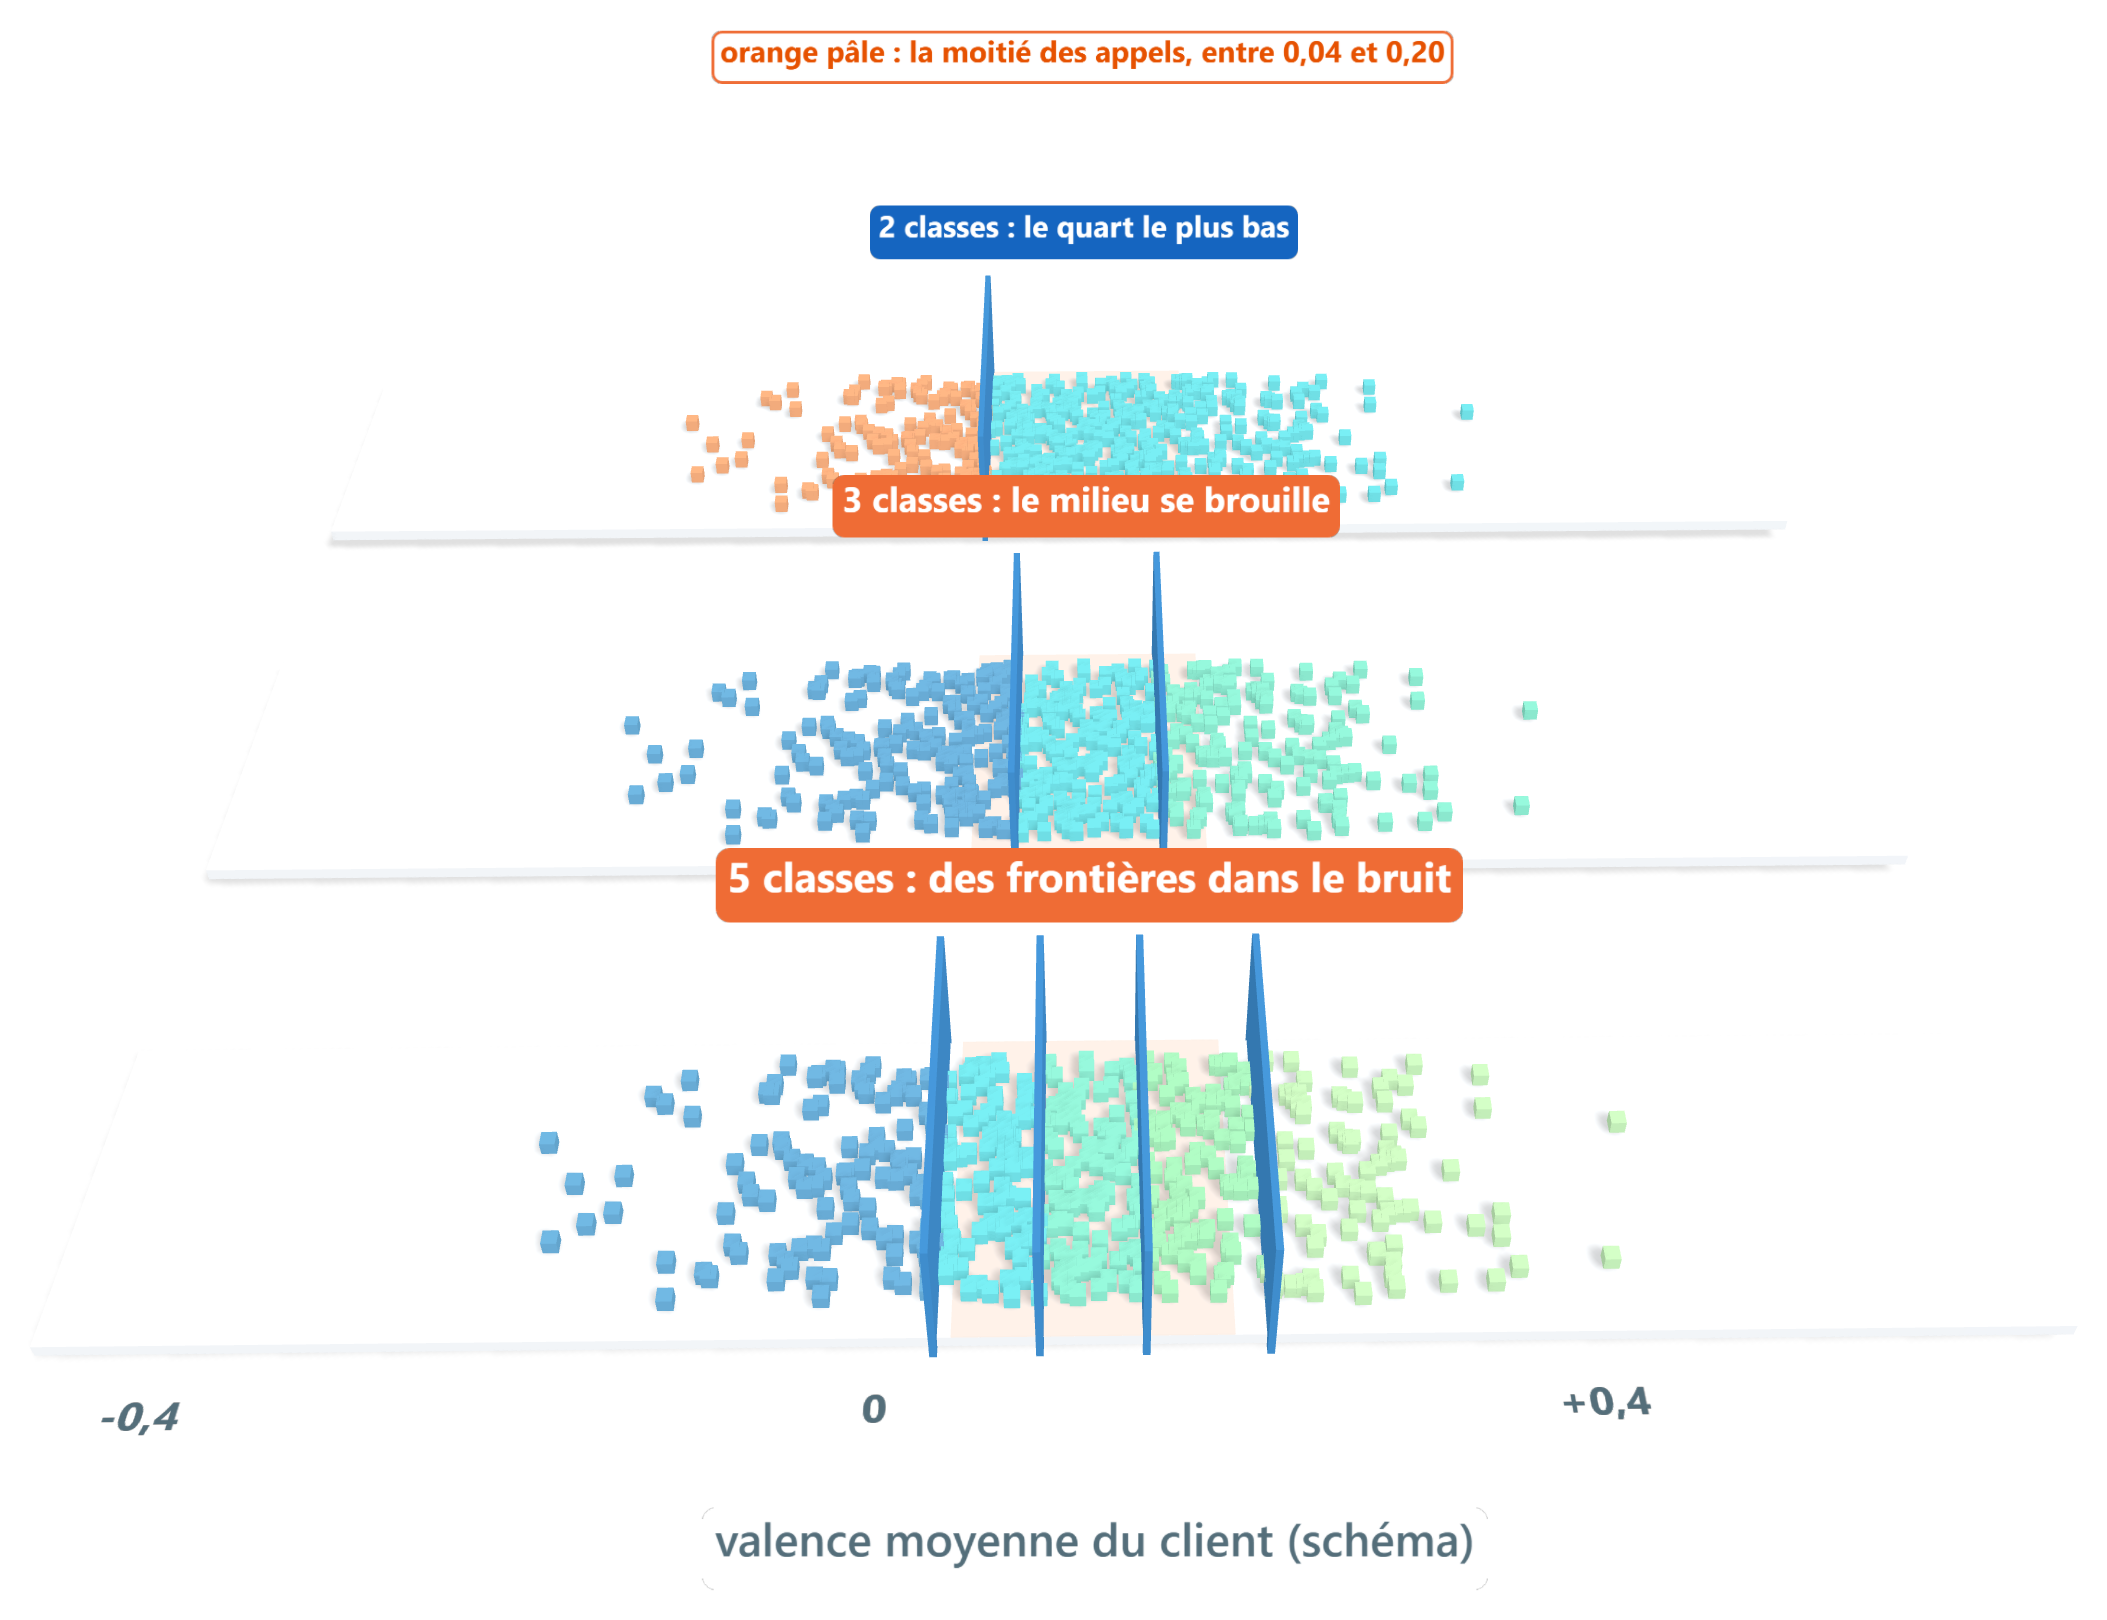
\includegraphics[width=0.72\linewidth]{3d_coupes.png}
\end{center}

\begin{tcbraster}[raster columns=3, raster equal height, raster column skip=6pt]
\begin{kpibox}[title={2 classes}, unbreakable]
\small AUC \textbf{0,849} : le quart le plus bas se reconnaît.
\end{kpibox}
\begin{kpibox}[title={3 classes}, colframe=orange!80!red, colbacktitle=orange!80!red, unbreakable]
\small extrêmes : AUC \textbf{0,85} ; milieu : \textbf{0,66}, presque au niveau du motif seul.
\end{kpibox}
\begin{kpibox}[title={5 classes}, colframe=orange!80!red, colbacktitle=orange!80!red, unbreakable]
\small 40\,\% de bonnes réponses ; \og plutôt bas \fg{} ou \og plutôt haut \fg{}, pas mieux.
\end{kpibox}
\end{tcbraster}

\begin{enfant}
\textbf{Ranger des enfants presque de la même taille en cinq rangs} : on repère les plus grands et les
plus petits, mais au milieu, c'est le hasard qui décide. Plus de rangs, ce n'est pas plus
d'information, ce sont plus de frontières arbitraires.
\end{enfant}

\section{La branche A bis : les modèles déjà entraînés}

\begin{center}
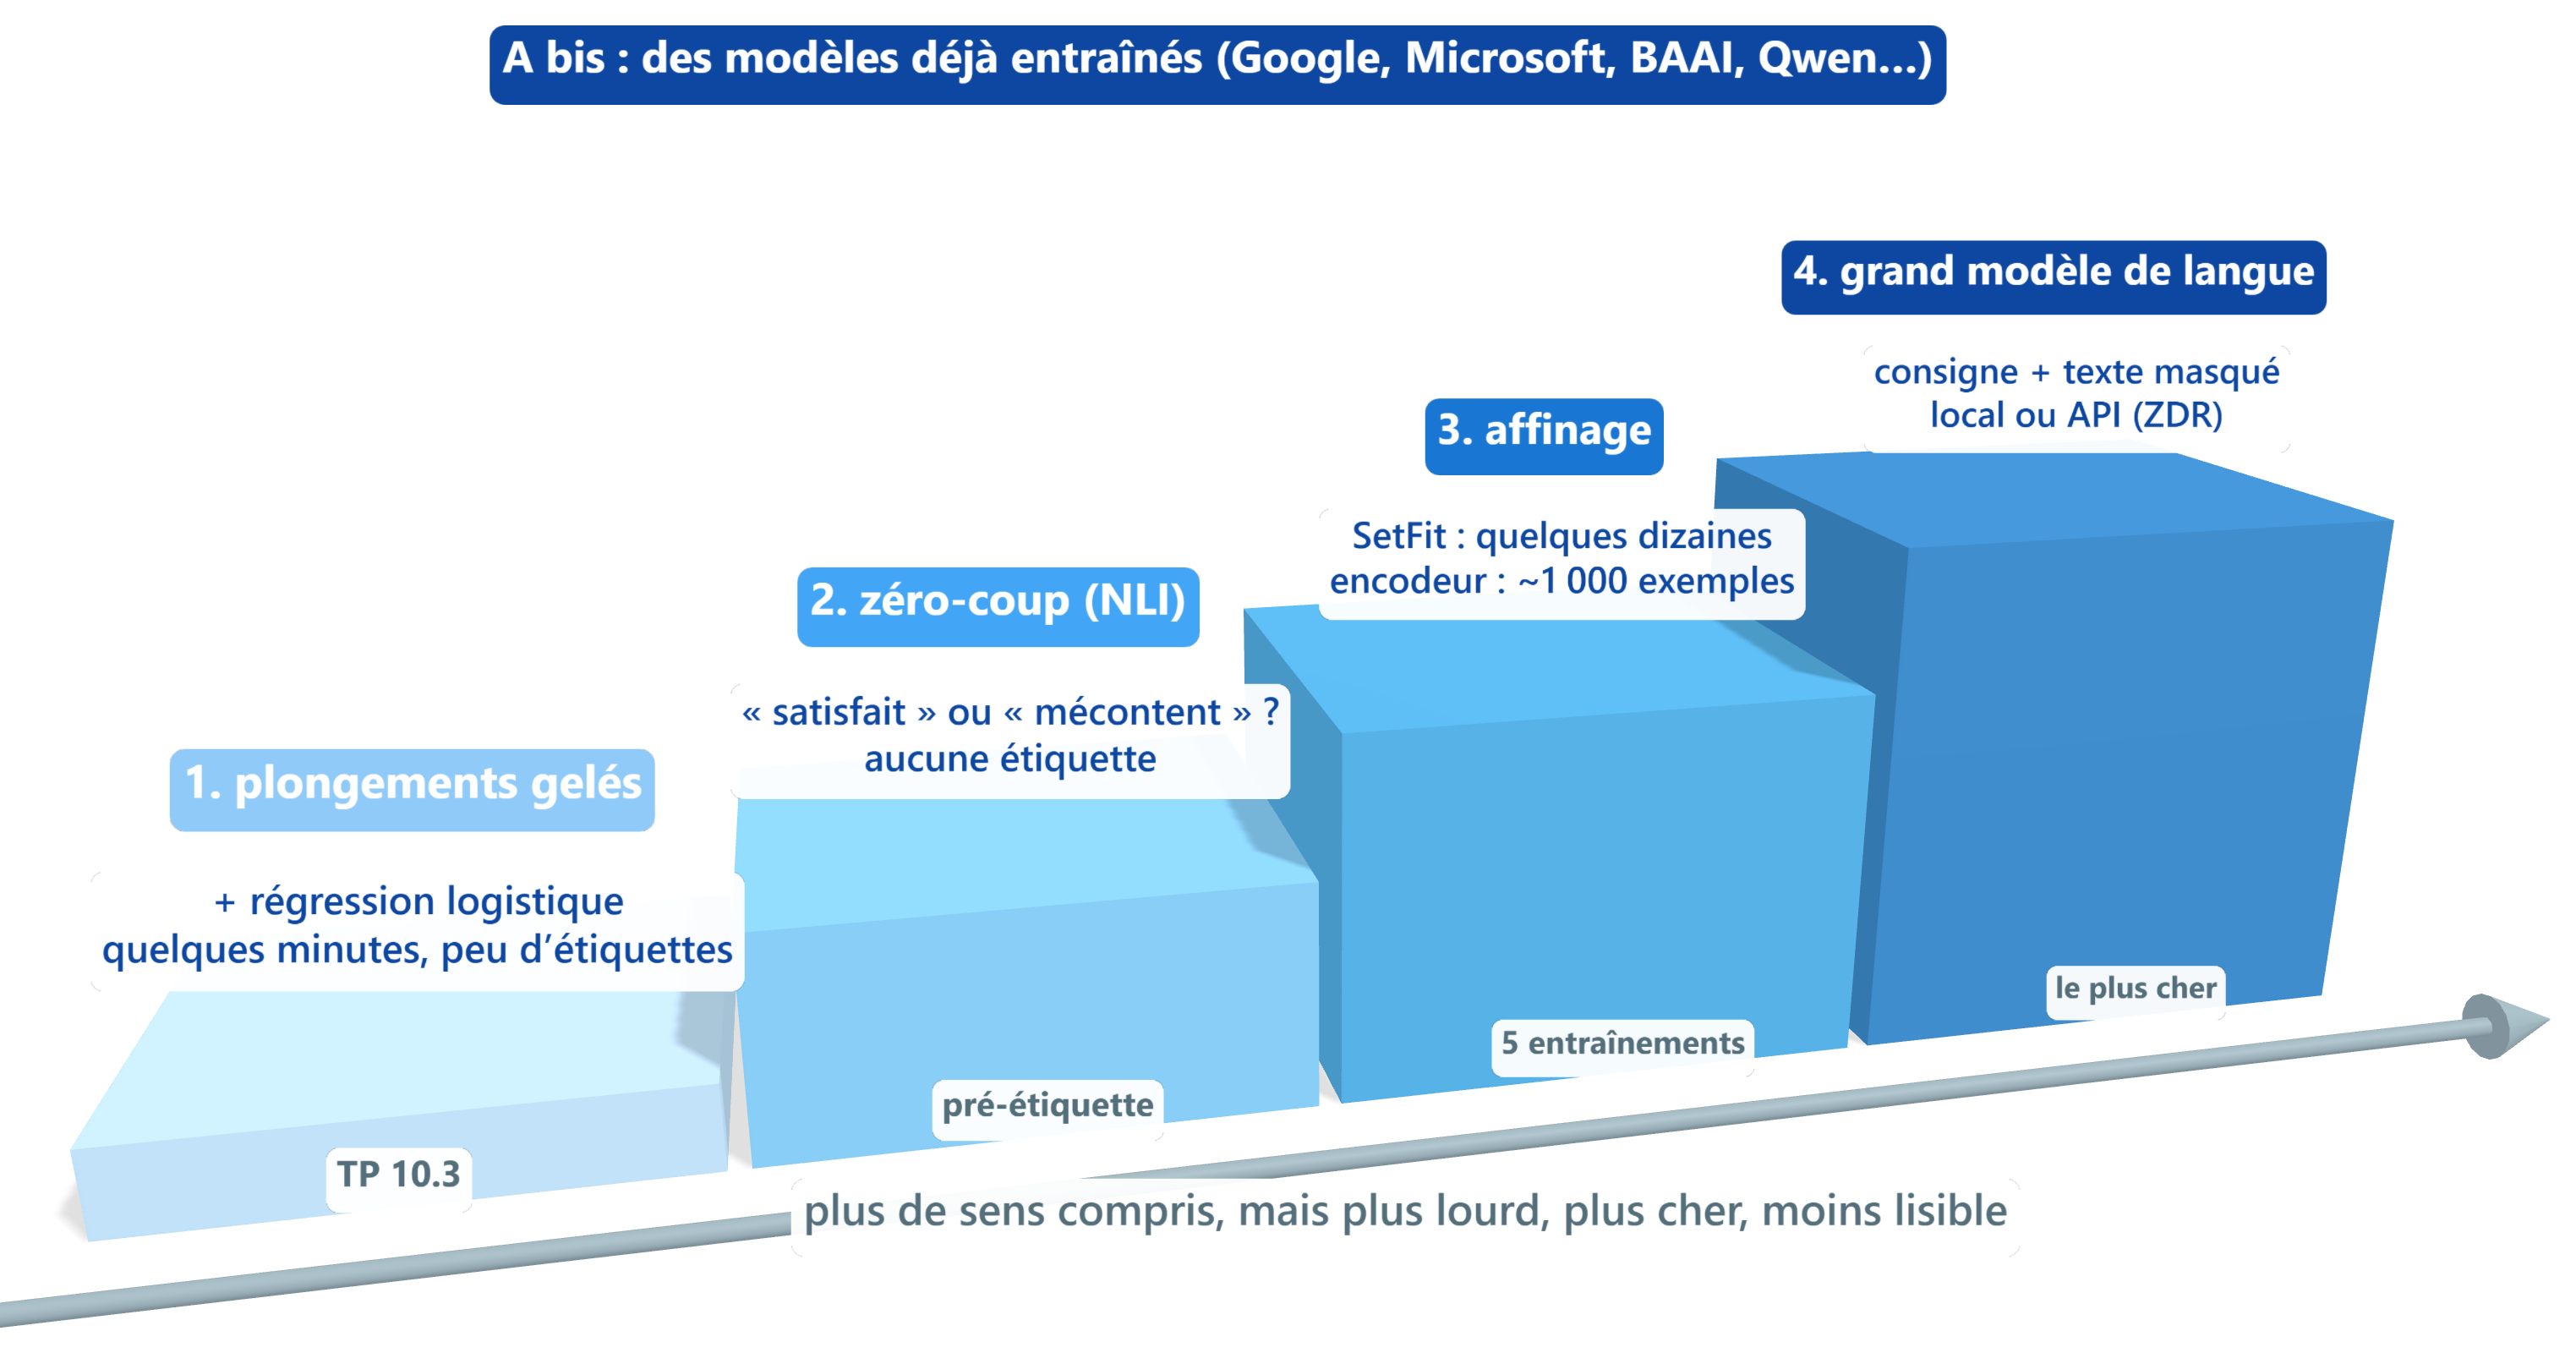
\includegraphics[width=0.85\linewidth]{3d_escalier.png}
\end{center}

\begin{tcbraster}[raster columns=2, raster equal height, raster column skip=8pt]
\begin{kpibox}[title={1. Plongements gelés (exercice 10.3)}, unbreakable]
\small un modèle de phrases donne un vecteur de \textbf{sens} par appel, puis la même régression
logistique. Pour le français : \texttt{intfloat/multilingual-e5-base}.
\end{kpibox}
\begin{kpibox}[title={2. Zéro-coup}, unbreakable]
\small \og satisfait \fg{} ou \og mécontent \fg{} ? sans aucune étiquette. Une \textbf{pré-étiquette},
pas une branche.
\end{kpibox}
\begin{kpibox}[title={3. Affinage}, unbreakable]
\small SetFit avec quelques dizaines d'exemples ; un encodeur complet avec un millier. \textbf{Un
entraînement par pli.}
\end{kpibox}
\begin{kpibox}[title={4. Grand modèle de langue}, unbreakable]
\small une consigne + le texte \textbf{masqué}. Le plus puissant, le plus cher ; il se juge comme un outil
de sentiment.
\end{kpibox}
\end{tcbraster}

\begin{stepbox}[title={\faPlug\quad La brancher}]
A bis donne \texttt{scores\_A2}, un score par appel, comme toutes les branches : fusion, ablation,
bootstrap, sans rien changer d'autre.\par\smallskip
\textbf{La seule question :} apporte-t-elle quelque chose que le TF-IDF n'a pas ?
\end{stepbox}

\begin{enfant}
\textbf{Le TF-IDF compte les mots ; un modèle pré-entraîné a déjà lu des milliards de phrases.} Il sait
que \og merci beaucoup \fg{} et \og c'est très gentil \fg{} veulent presque dire la même chose.
\end{enfant}

\subsection*{Le match : TF-IDF contre Google contre Qwen}

\begin{center}
\begin{tikzpicture}[
  r/.style={draw=#1, fill=#1!10, rounded corners=6pt, text width=3.3cm, align=center, font=\small,
    minimum height=1.2cm, inner sep=4pt},
  fl/.style={-{Stealth[length=2.5mm]}, thick, color=slate}]
\node[r=sectioncolor] (a) {\textbf{TF-IDF}\\(la branche A)};
\node[r=darkblue, below=0.25cm of a] (g) {\textbf{Google}\\{\scriptsize\texttt{embeddinggemma-300m}}};
\node[r=accentblue, below=0.25cm of g] (q) {\textbf{Qwen}\\{\scriptsize\texttt{Qwen3-Embedding-0.6B}}};
\node[draw=darkblue, fill=notebg, rounded corners=6pt, text width=3.0cm, align=center, font=\small, minimum height=4.2cm, right=1.0cm of g] (lr) {\textbf{même texte masqué}\\\textbf{même classifieur}\\\textbf{mêmes plis}};
\node[draw=orange!80!red, fill=orange!8, rounded corners=6pt, text width=3.6cm, align=center, font=\small, minimum height=4.2cm, right=1.0cm of lr] (v) {\textbf{verdict}\\[3pt]gain sur le TF-IDF, avec son intervalle\\[3pt]borne basse $> 0$ ?\\oui : on change\\non : on garde le TF-IDF};
\foreach \n in {a,g,q} \draw[fl] (\n) -- (lr.west |- \n);
\draw[fl, very thick] (lr) -- (v);
\end{tikzpicture}
\end{center}

\begin{piege}
\textbf{Ni \og le meilleur score \fg{}, ni \og la moyenne \fg{}.} Garder le meilleur des trois, c'est
garder le lancer de dé chanceux ; la moyenne donne le même poids au médiocre qu'au bon. On change
seulement si le gain est \textbf{net} (bootstrap apparié), et la \textbf{fusion apprise} pondère elle-même
les représentations ; elle n'est gardée que si elle bat nettement la meilleure seule.
\end{piege}

\begin{piege}
\textbf{Pourquoi pas tout de suite un réseau de neurones ?} Avec 1\,446 appels, ce modèle simple est
difficile à battre, il s'entraîne en une seconde, et ses poids se lisent. On ne sait si un modèle plus
gros apporte quelque chose qu'en le comparant à celui-ci.
\end{piege}

% Copyright (c) 2026 Selina Cheggour. Tous droits réservés. Voir le fichier LICENSE.
% Fiche 4 : séance 3 du TP (parties 5 et 6 : la voix, le déroulement).

\bandeaupartie{Fiche 4 : séance 3}{La voix et le déroulement : deux branches qui ne lisent pas les mots.}

\section{Branche B : comment c'est dit}

\begin{center}
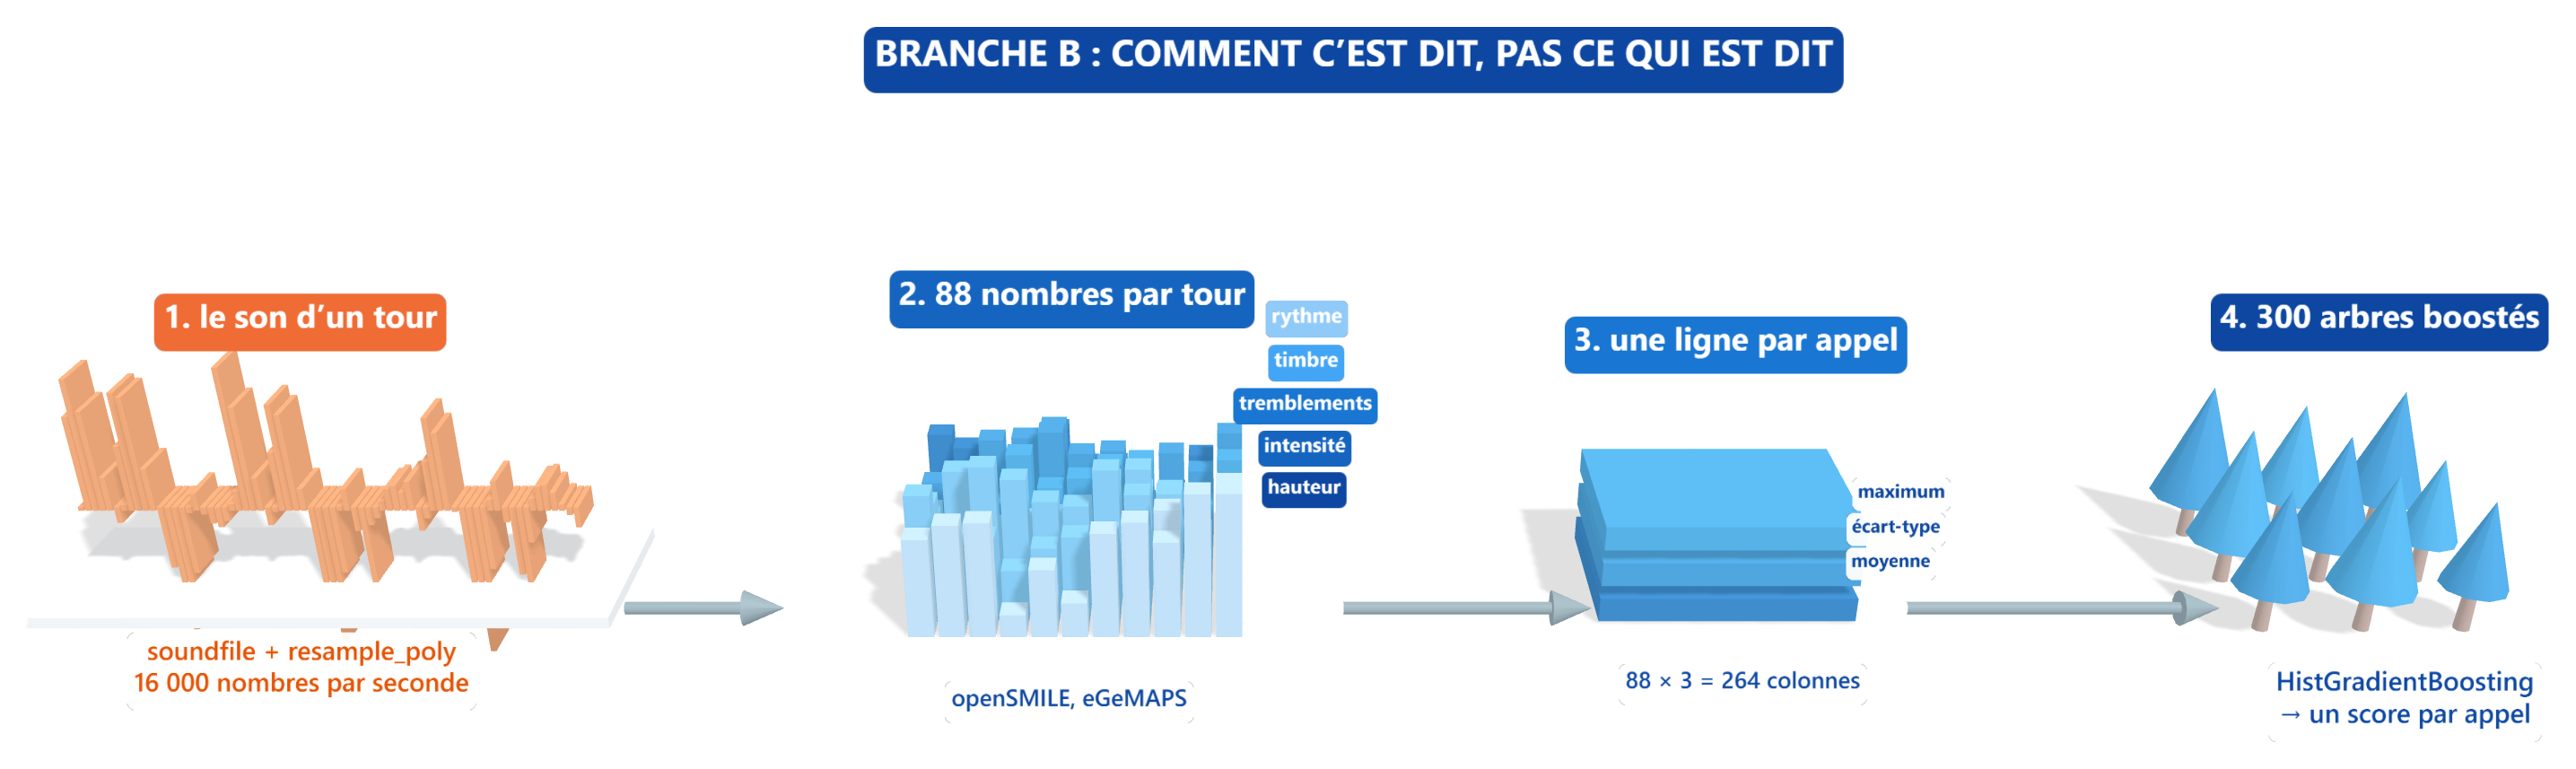
\includegraphics[width=\linewidth]{3d_voix.png}
\end{center}

\begin{enfant}
\textbf{Écouter quelqu'un parler une langue qu'on ne comprend pas} : on devine quand même s'il est fâché,
à sa voix.
\end{enfant}

\begin{stepbox}[title={5.1 à 5.3\quad Du son à une ligne par appel}]
\begin{tabularx}{\linewidth}{>{\bfseries\color{sectioncolor}}c X >{\raggedright\arraybackslash}p{4.9cm}}
5.1 & \texttt{signal\_du\_tour} : la tranche du tour, de 8\,000 à 16\,000~Hz & \faCheckCircle\ 4,08~s \faArrowRight\ \textbf{65\,280} nombres \\
5.2 & \texttt{descripteurs} : openSMILE, eGeMAPS & \faCheckCircle\ \textbf{88} valeurs par tour \\
5.3 & \texttt{X\_B} : moyenne, écart-type, maximum par appel & \faCheckCircle\ \textbf{1\,446} $\times$ \textbf{264} \\
\end{tabularx}
\end{stepbox}

\begin{tcbraster}[raster columns=5, raster equal height, raster column skip=4pt]
\begin{kpibox}[title={hauteur}, unbreakable, fonttitle=\bfseries\footnotesize, left=4pt, right=4pt]\scriptsize grave ou aiguë, monocorde ou chantante\end{kpibox}
\begin{kpibox}[title={intensité}, unbreakable, fonttitle=\bfseries\footnotesize, left=4pt, right=4pt]\scriptsize forte ou faible\end{kpibox}
\begin{kpibox}[title={\scriptsize tremblements}, lefttitle=2pt, righttitle=2pt, unbreakable, fonttitle=\bfseries\footnotesize, left=4pt, right=4pt]\scriptsize jitter, shimmer : la voix qui chevrote\end{kpibox}
\begin{kpibox}[title={timbre}, unbreakable, fonttitle=\bfseries\footnotesize, left=4pt, right=4pt]\scriptsize claire ou sourde, souffle\end{kpibox}
\begin{kpibox}[title={rythme}, unbreakable, fonttitle=\bfseries\footnotesize, left=4pt, right=4pt]\scriptsize morceaux voisés, pauses\end{kpibox}
\end{tcbraster}

\begin{stepbox}[title={5.4\quad Classer, et comparer deux découpages}]
\texttt{HistGradientBoostingClassifier} : 300 petits arbres, chacun corrige les erreurs du précédent.
\doisvoir{par locuteur \textbf{0,53} \quad au hasard \textbf{0,70}}
\end{stepbox}

\begin{piege}
\textbf{0,70 au hasard, c'est un mirage.} Les 88 descripteurs reconnaissent la personne dans \textbf{97\,\%}
des cas (exercice~5.5) : au hasard, le modèle reconnaît des voix, pas une humeur. \textbf{Toujours
séparer les personnes} entre entraînement et test.
\end{piege}

\section{Branche C : la forme de la conversation}

\begin{center}
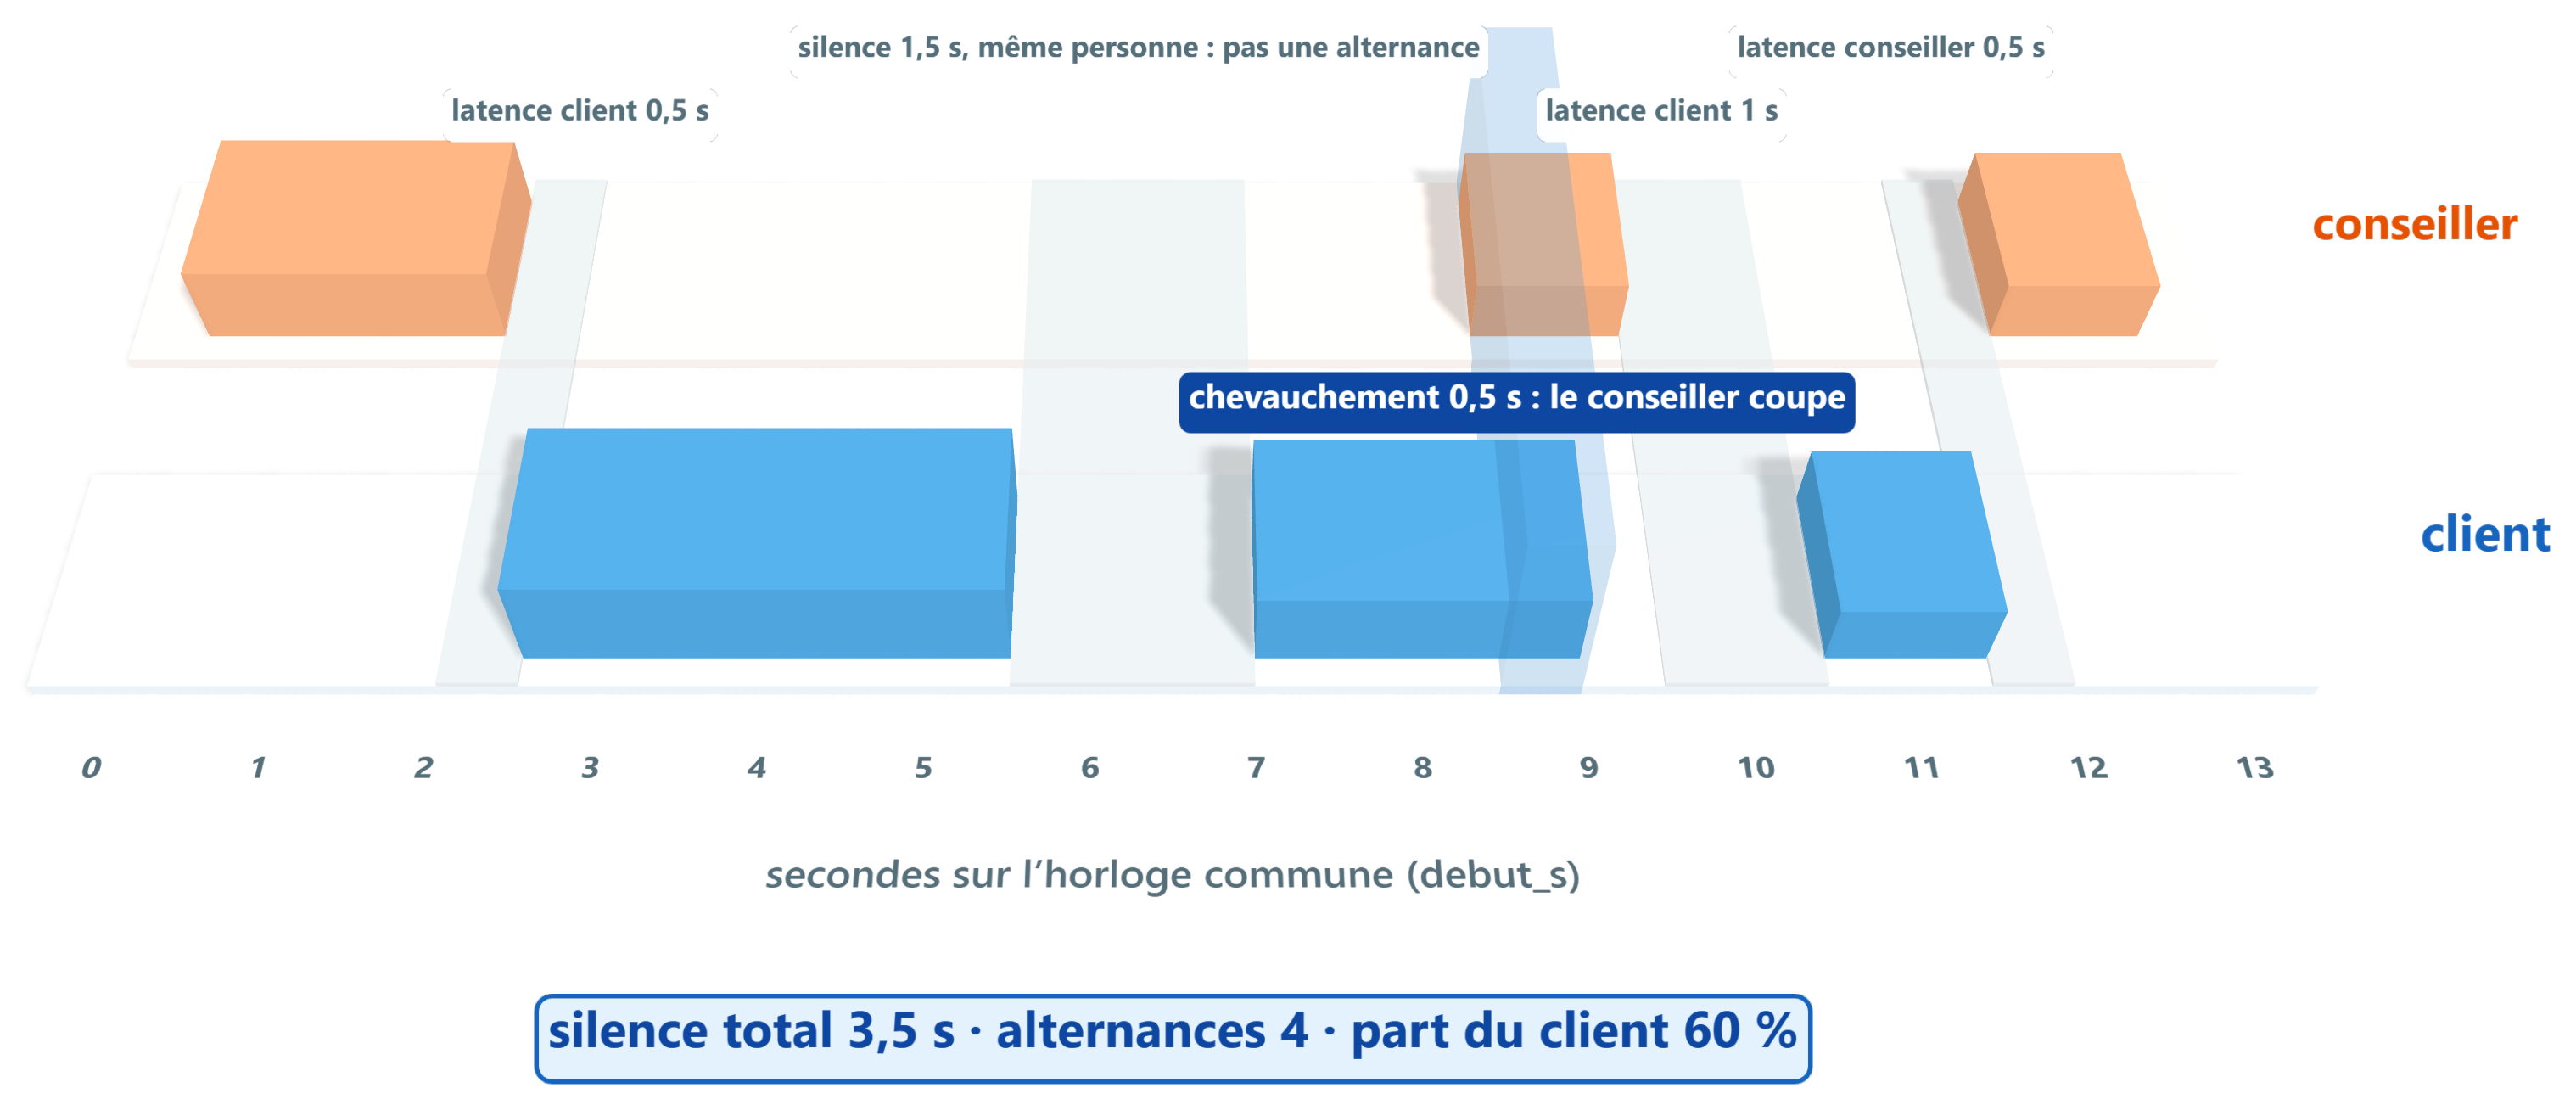
\includegraphics[width=\linewidth]{3d_deroulement.png}
\end{center}

\begin{enfant}
\textbf{Regarder un match de ping-pong sans voir la balle} : au rythme des coups et des pauses, on devine si
la partie est fluide ou chaotique.
\end{enfant}

\begin{stepbox}[title={6.1\quad Les 14 indicateurs, d'abord à la main sur l'appel ci-dessus}]
\textbf{écart} = début du tour suivant $-$ fin du tour : \textbf{positif} = silence, \textbf{négatif} =
chevauchement. Deux personnes différentes = une \textbf{alternance}.
\doisvoir{silence total \textbf{3,5~s}, alternances \textbf{4}, chevauchement \textbf{0,5~s}, part du client
\textbf{0,6}, latence du client \textbf{0,75~s}.}
\end{stepbox}

\begin{piege}
\textbf{Le piège :} un silence entre deux tours de la \emph{même} personne est un silence, mais
\textbf{pas} une alternance.
\end{piege}

\begin{stepbox}[title={6.2 et 6.3\quad Le tableau, puis le classifieur}]
14 indicateurs + attente + durée = \textbf{16 colonnes}, le même classifieur que la voix, le même découpage.
\doisvoir{\texttt{X\_C} de \textbf{1\,446} $\times$ \textbf{16}, puis AUC proche de \textbf{0,61} (repère
\og motif seul \fg{} : 0,637).}
\end{stepbox}

\begin{center}
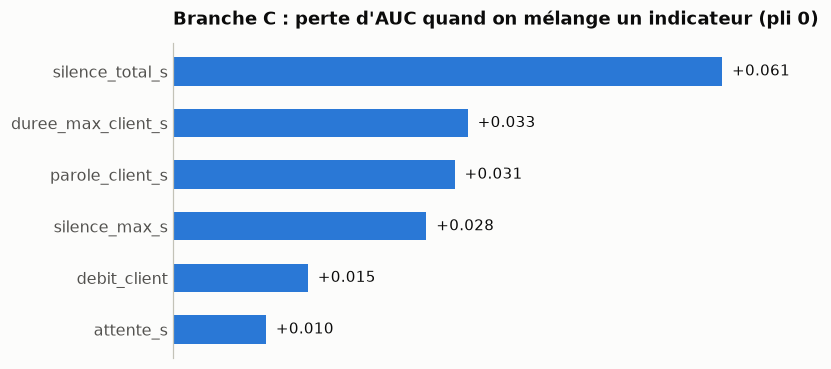
\includegraphics[width=0.62\linewidth]{tp_importance_C.png}
\end{center}

\begin{tcbraster}[raster columns=2, raster equal height, raster column skip=8pt]
\begin{kpibox}[title={\faSearch\ Ce que regarde le modèle}, unbreakable]
\small Le silence total et la longueur des tours : la \textbf{durée de la tâche}, pas l'humeur. Payer une
facture fait 43~s de silences, demander les horaires 15~s.
\end{kpibox}
\begin{kpibox}[title={\faRandom\ L'importance par permutation}, unbreakable]
\small On mélange une colonne et on regarde si le score baisse.
\image{On remplace un ingrédient par n'importe quoi et on goûte.}
\end{kpibox}
\end{tcbraster}

\section{Pourquoi ne pas prendre directement les \og bis \fg{} ?}

\begin{center}
\begin{tikzpicture}[
  r/.style={draw=#1, fill=#1!10, rounded corners=6pt, text width=3.1cm, align=center, font=\small,
    minimum height=1.25cm, inner sep=4pt},
  fl/.style={-{Stealth[length=2.5mm]}, thick, color=slate}]
\node[r=sectioncolor] (s) {\textbf{simple}\\TF-IDF, eGeMAPS};
\node[r=darkblue, below=0.4cm of s] (b) {\textbf{bis}\\Google, Qwen, wav2vec};
\node[draw=orange!80!red, fill=orange!8, rounded corners=6pt, text width=3.5cm, align=center, font=\small, minimum height=3.0cm, right=1.1cm of s, yshift=-0.85cm] (c) {\textbf{le même classifieur}\\entraîné sur \textbf{tes} appels};
\node[r=accentblue, right=1.0cm of c] (sc) {\textbf{un score}};
\draw[fl] (s) -- (c.west |- s); \draw[fl] (b) -- (c.west |- b); \draw[fl, very thick] (c) -- (sc);
\end{tikzpicture}
\end{center}

\begin{tcbraster}[raster columns=3, raster equal height, raster column skip=6pt]
\begin{kpibox}[title={\faGraduationCap\ Il faut apprendre}, unbreakable]
\small Un modèle de Google ne sait pas ce qu'est un client mécontent \emph{dans cette entreprise} : le classifieur
derrière s'entraîne sur tes appels, simple ou bis.
\end{kpibox}
\begin{kpibox}[title={\faBalanceScale\ Le simple est le témoin}, unbreakable]
\small 0,80 pour Google ne veut rien dire si le simple fait 0,79. Et seul le simple se lit.
\end{kpibox}
\begin{kpibox}[title={\faTools\ Le bis casse plus}, unbreakable]
\small carte graphique, versions, jetons, licences, 512 jetons, modèle anglais. Les erreurs de données
touchent les deux pareil.
\end{kpibox}
\end{tcbraster}

\begin{enfant}
\textbf{Un dictionnaire très savant ne sait pas corriger ton contrôle} : il faut encore lui montrer des
copies corrigées.
\end{enfant}

\begin{stepbox}[title={\faRoute\quad La règle}]
\textbf{Le simple d'abord} (le repère), \textbf{le bis ensuite} (même cellule, test apparié). Le bis
gagne nettement ? on le garde. Sinon, on garde le simple, sans carte graphique, avec la preuve chiffrée.
\end{stepbox}


\end{document}
